\documentclass{article}
\usepackage{graphicx}
\usepackage[margin=1in]{geometry}
\usepackage{amsmath}
\usepackage{amssymb}
\usepackage{amsthm}
\usepackage{booktabs}
\usepackage{enumitem}
\usepackage{hyperref}
\usepackage{float}
\emergencystretch=3em
\title{Aryan K STAT 37711 PS2}
\author{Aryan Kaushal}
\begin{document}
\maketitle

\section*{Problem 1}
Code at: \url{https://github.com/aryankaushal06/STAT-37711-A26-PSet-Code/blob/main/PS2/p1.py}

\begin{enumerate}[label=\alph*.]
\item Let $g(x)=(a(x),b(x))\in\mathbb{R}^2$ be the raw network output

Set $f_\mu(x)=a(x)$ and $f_\sigma(x)=\log(1+e^{b(x)})+\epsilon$, with $\epsilon>0$ a fixed small constant

The identity link imposes no restriction on a conditional mean, while the softplus link guarantees a strictly positive conditional standard deviation, as required for a nondegenerate Normal density

\item For observations $(x_i,y_i)$, assume conditionally independent responses $Y_i\mid X_i=x_i\sim\mathcal N(\mu_i,\sigma_i^2)$, where $\mu_i=f_\mu(x_i)$ and $\sigma_i=f_\sigma(x_i)>0$

The conditional density is $p(y_i\mid x_i)=\frac{1}{\sqrt{2\pi}\sigma_i}\exp\!\left(-\frac{(y_i-\mu_i)^2}{2\sigma_i^2}\right)$

Thus the empirical negative log-likelihood to minimize is $\mathcal L=\frac{1}{n}\sum\limits_{i=1}^{n}\left[\frac{1}{2}\log(2\pi)+\log\sigma_i+\frac{(y_i-\mu_i)^2}{2\sigma_i^2}\right]$

The $\log\sigma_i$ term penalizes declaring excessive uncertainty, while the standardized squared-residual term penalizes declaring too little uncertainty at an observation with a large residual

Unlike homoscedastic least squares, this objective learns both the conditional location and the input-dependent noise scale

\item \textbf{Data:} \texttt{taxi\_trips.parquet} has $523554$ rows and the $8$ expected columns, with no missing or nonfinite values and no nonpositive durations, so no rows are removed

The duration has median $8.63$, mean $10.41$, standard deviation $7.75$, $99.9$th percentile $63.27$, and maximum $227.94$ minutes, and $99.560\%$ of trips last under $45$ minutes

\textbf{Splits:} I partition rows at random with seed $42$ into $366487$ training ($70\%$), $78533$ validation ($15\%$), and $78534$ test ($15\%$) rows

The supplied features were standardized on the whole file; the additional affine scaler in the code is fitted on the training partition only

\textbf{Model:} The network is a ReLU MLP on the $7$ features with $2$ outputs, transformed by the links in (a) with $\epsilon=10^{-3}$

The output bias starts at the training mean and the inverse softplus of the training standard deviation

\textbf{Training:} I minimize the NLL in (b) with AdamW (learning rate $10^{-3}$, weight decay $10^{-4}$), batch size $2048$, and gradient-norm clipping at $10$, for at most $200$ epochs

Early stopping monitors validation NLL with patience $15$ and restores the best parameters

The hidden layers are chosen by minimum validation NLL, as in the table below; the test set played no part

\begin{table}[H]
\centering
\begin{tabular}{lccc}
\toprule
Hidden layers & Restored epoch & Epochs run & Validation NLL \\
\midrule
$(64,64)$ & 147 & 162 & 2.6134 \\
$(128,128)$ & 60 & 75 & 2.5957 \\
$(256,256,256)$ & 30 & 45 & \textbf{2.5788} \\
\bottomrule
\end{tabular}
\caption{Architecture selection on the validation set}
\end{table}

\textbf{Baselines:} All are fitted on training data: a constant probability $\hat p_0=\frac{1}{n_{\mathrm{train}}}\sum\limits_{i\in\mathrm{train}}\mathbf 1\{y_i<45\}=0.99559$, and a constant Gaussian with $\hat\mu=10.416$ and $\hat\sigma=7.755$

I add a homoscedastic MLP with the selected architecture and one learned $\sigma$ (restored epoch $50$, validation NLL $2.7068$), which isolates the value of an input-dependent $\sigma(x)$

\textbf{Numerical stability:} Training raises an error on any nonfinite loss or gradient norm, and none occurred

The figure below shows that instability is confined to the start: epoch $1$ has mean training NLL $2486$ and a maximum gradient norm of $6.36\times 10^{6}$, after which norms stay near the clipping threshold or below it; over the whole run $0.14\%$ of steps were clipped

On test inputs $\hat\sigma(x)$ ranges from $0.65$ to $28.85$ minutes with median $3.10$, so it is always positive and never reaches the floor $\epsilon$

\begin{figure}[H]\centering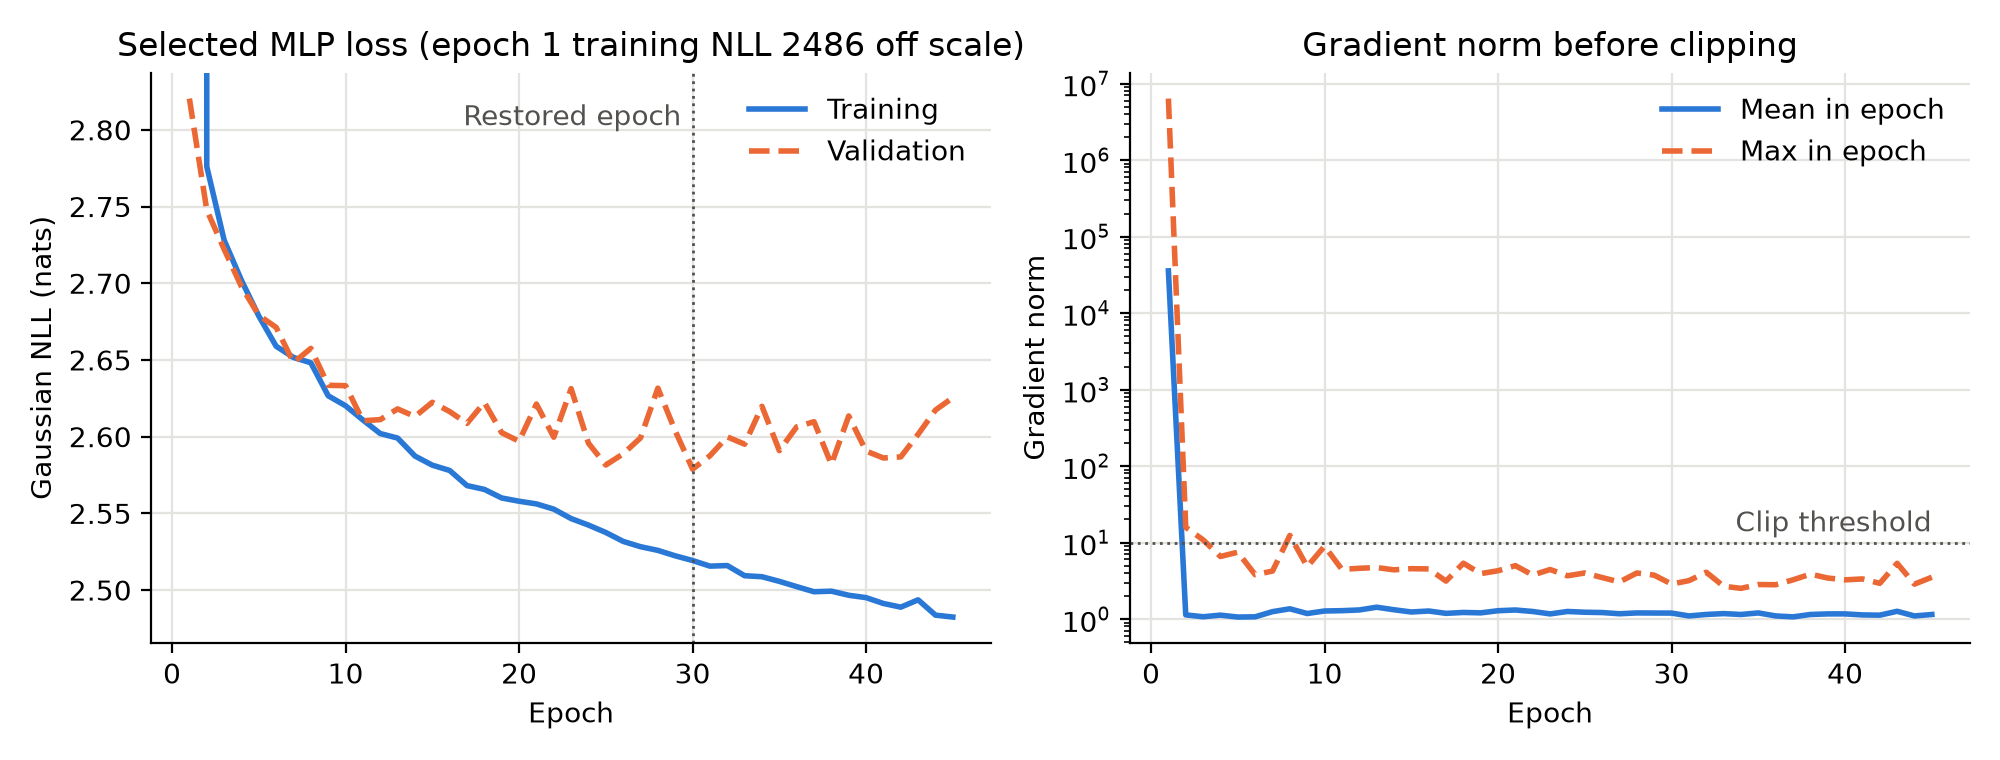
\includegraphics[width=\textwidth]{figures/p1_training.png}\caption{Training diagnostics for the selected MLP; validation NLL flattens near epoch $10$ while training NLL keeps falling}\end{figure}

\textbf{Fit:} The MLP's mean has test RMSE $3.875$ and MAE $2.372$ minutes, against $7.757$ and $5.682$ for the constant mean

The figure below shows that the predicted noise grows with the predicted mean, so the data are visibly heteroscedastic

\begin{figure}[H]\centering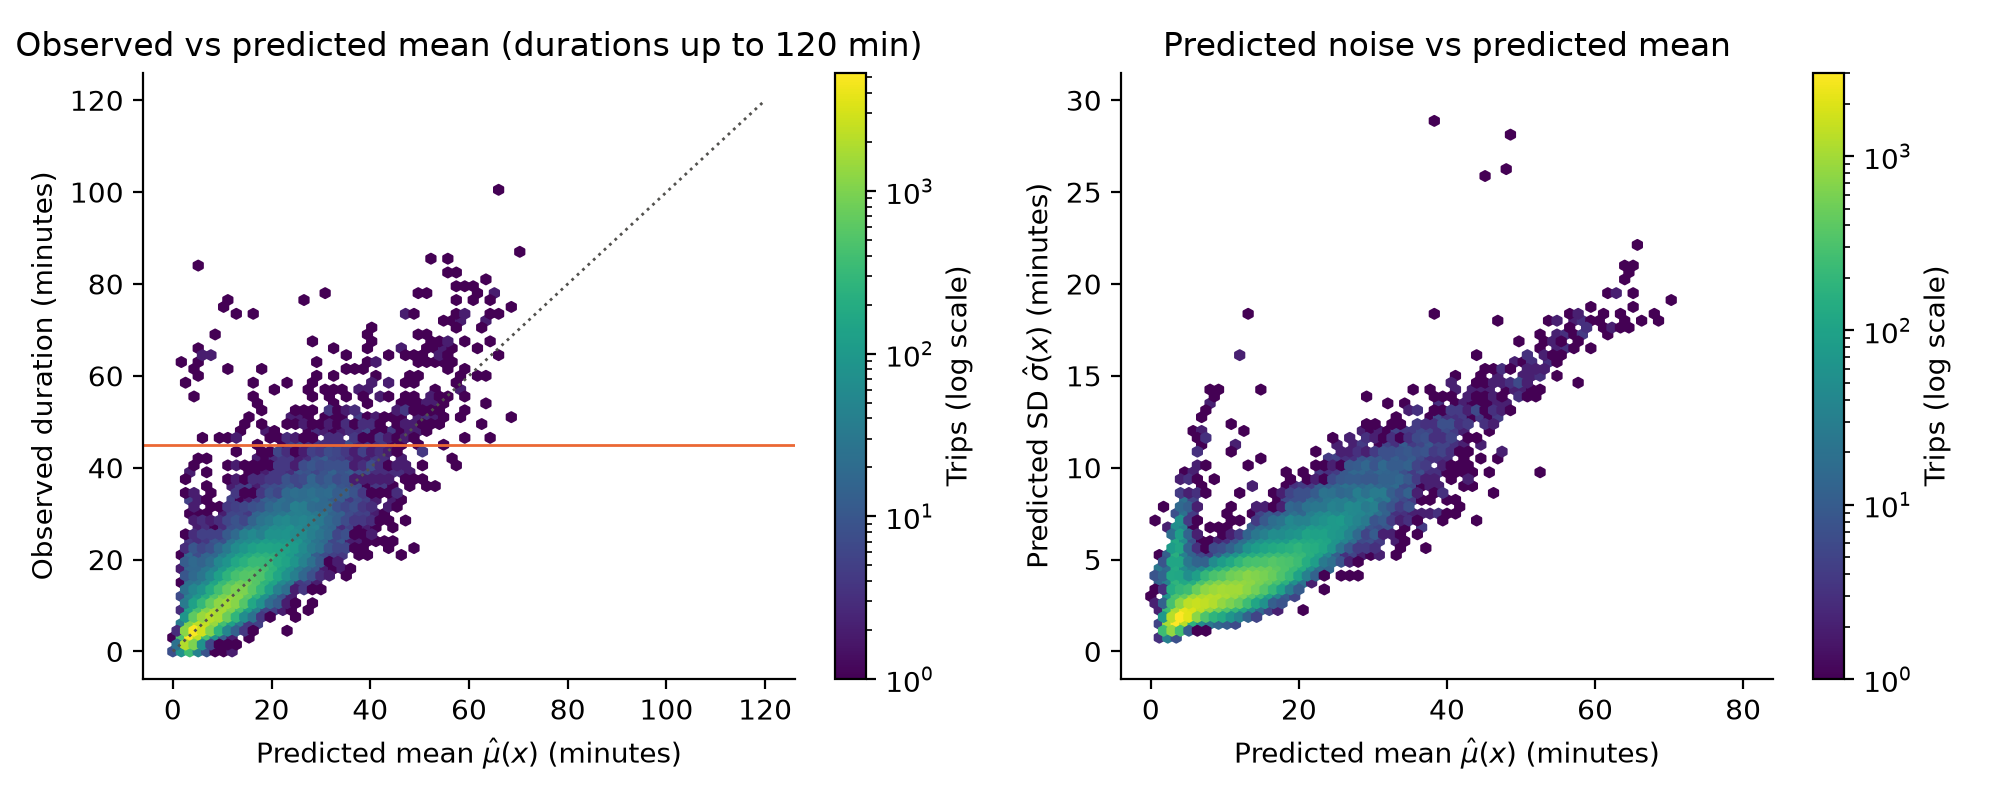
\includegraphics[width=\textwidth]{figures/p1_pred_vs_obs.png}\caption{Test-set predictions; the orange line marks $45$ minutes, and the left panel omits durations above $120$ minutes}\end{figure}

\item Given input $x$ and fitted $\hat\mu(x)$, $\hat\sigma(x)>0$, the desired probability is $P(Y<45\mid X=x)=\Phi\!\left(\frac{45-\hat\mu(x)}{\hat\sigma(x)}\right)$, where $\Phi$ is the standard Normal CDF

This follows by standardizing $Z=\frac{Y-\hat\mu(x)}{\hat\sigma(x)}\sim\mathcal N(0,1)$ under the fitted model

The code evaluates this CDF with \texttt{ndtr} and the logarithm of both tails with \texttt{log\_ndtr}, both from \texttt{scipy.special}, so it predicts probabilities rather than hard labels or mean travel times

\item Define $z_i=\mathbf 1\{y_i<45\}$ and $\hat p_i=\Phi\!\left(\frac{45-\hat\mu(x_i)}{\hat\sigma(x_i)}\right)$ for held-out test observations

The Brier score is $\operatorname{Brier}=\frac{1}{m}\sum\limits_{i=1}^{m}(\hat p_i-z_i)^2$, and the binary log-loss is $\operatorname{LogLoss}=-\frac{1}{m}\sum\limits_{i=1}^{m}[z_i\log\hat p_i+(1-z_i)\log(1-\hat p_i)]$

Both are proper scoring rules, so in expectation they favor calibrated probabilities reflecting the true event probabilities

The requested thresholded accuracy is $\operatorname{Accuracy}=\frac{1}{m}\sum\limits_{i=1}^{m}\mathbf 1\{\mathbf 1\{\hat p_i\geq 0.5\}=z_i\}$

I report the exact log-loss, computed from $\log\Phi$ without clipping, and a clipped version with each $\hat p_i$ restricted to $[10^{-7},1-10^{-7}]$

\begin{table}[H]
\centering
\begin{tabular}{lccccc}
\toprule
Model & Brier & Log-loss & Clipped log-loss & Accuracy & Gaussian NLL \\
\midrule
Heteroscedastic MLP & 0.002717 & 0.05186 & 0.01707 & 0.99680 & 2.7654 \\
Homoscedastic MLP & 0.002568 & 0.04001 & 0.02174 & 0.99708 & 2.7424 \\
Constant Gaussian & 0.004457 & 0.05528 & 0.05528 & 0.99554 & 3.4675 \\
Constant probability & 0.004437 & 0.02857 & 0.02857 & 0.99554 & --- \\
\bottomrule
\end{tabular}
\caption{Held-out test scores on the same $78534$ trips, seed $42$}
\end{table}

The heteroscedastic MLP has $\boxed{\operatorname{Brier}=0.002717}$, $\boxed{\operatorname{LogLoss}=0.05186}$, and $\boxed{\operatorname{Accuracy}=0.99680}$

\textbf{Accuracy:} Only $350$ test trips ($0.446\%$) last at least $45$ minutes, so always predicting ``under $45$'' already scores $0.99554$, which both constant baselines do

The heteroscedastic MLP flags $173$ trips as at least $45$ minutes, of which $136$ are correct, and so it finds $38.9\%$ of the long trips

\textbf{Brier:} The MLP improves on the constant probability by $38.8\%$, and the paired $95\%$ intervals for the difference exclude $0$ against both required baselines: $[-0.00202,-0.00142]$ against the constant probability and $[-0.00204,-0.00144]$ against the constant Gaussian

Against the homoscedastic MLP the interval is $[-0.000001,0.000299]$, so this difference is not established

\textbf{Log-loss:} The exact log-loss is worse than the constant probability's, with paired interval $[0.00199,0.04457]$, and its difference from the constant Gaussian is not established, with interval $[-0.02455,0.01772]$

This result is driven by a few rows: the median row loss is near $0$, the $10$ worst rows account for $55.4\%$ of the total, and the worst single row contributes $604.3$

Clipped log-loss limits each row to $-\log 10^{-7}$ and affects $36$ rows; on it the MLP beats the constant probability (interval $[-0.01402,-0.00897]$) and the homoscedastic MLP (interval $[-0.00624,-0.00310]$)

The clipped score is less sensitive to these rows but is not the model's actual log-loss, which is why I report both

\textbf{Gaussian NLL:} The MLP's test NLL of $2.7654$ exceeds its validation NLL of $2.5788$ and the homoscedastic MLP's test NLL of $2.7424$, because one row has an NLL of $9816.6$: a trip of $173.3$ minutes with $\hat\mu=2.85$ and $\hat\sigma=1.22$, a standardized residual of $140$

That row alone adds $0.125$ to the test mean

After dropping the worst $0.1\%$ of rows, the NLL is $2.4963$ on test and $2.4891$ on validation for this model, against $2.6276$ for the homoscedastic MLP and $3.4268$ for the constant Gaussian on test

\textbf{Calibration:} The figure below groups trips by predicted $P(Y\geq 45)$ and shows that $\hat\sigma(x)$ improves calibration in the tail

In the bin with predicted tail probability between $0.001$ and $0.003$, the event occurs at rate $0.00795$ for the heteroscedastic MLP and $0.09821$ for the homoscedastic MLP, against mean predictions of $0.00183$ and $0.00182$

Above a predicted tail probability of $0.01$ the heteroscedastic MLP tracks the diagonal closely, while below it the model understates the risk

\begin{figure}[H]\centering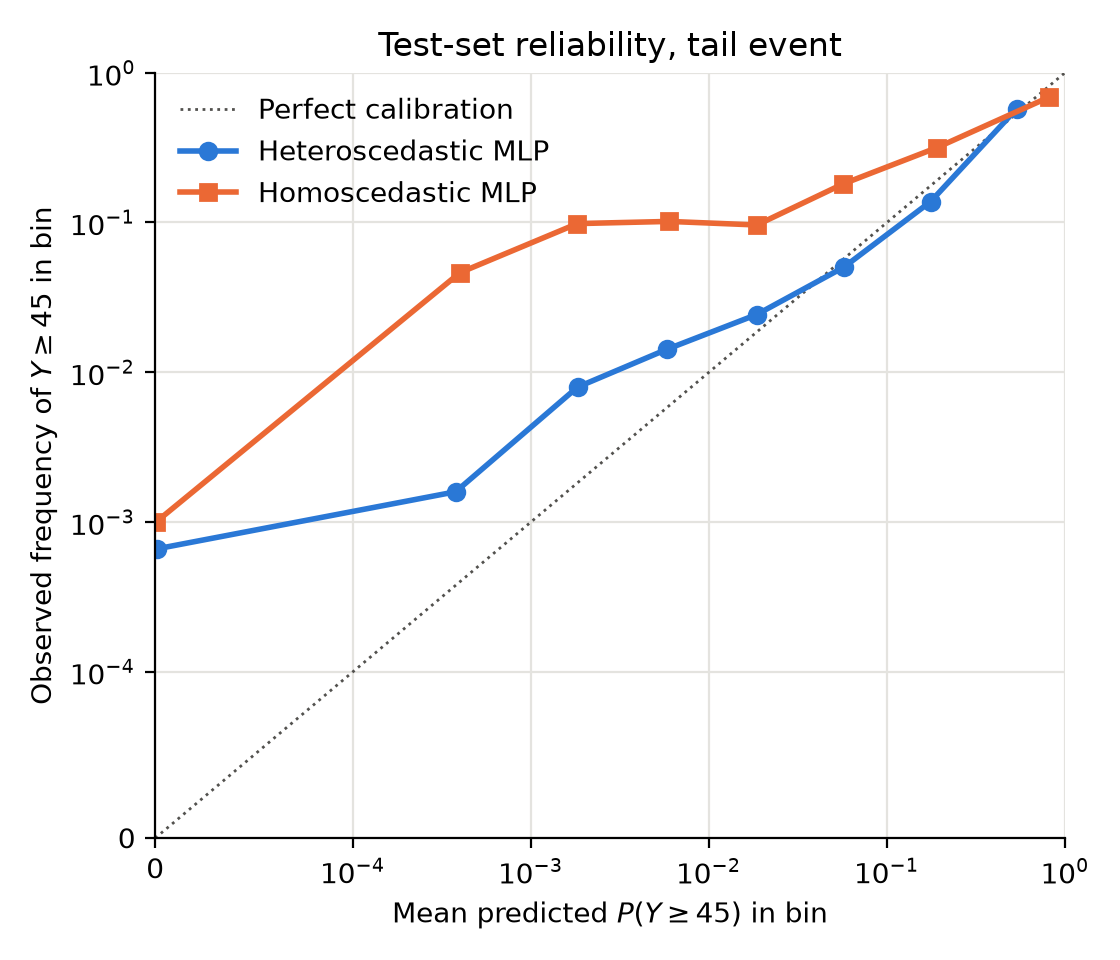
\includegraphics[width=.62\textwidth]{figures/p1_calibration.png}\caption{Test-set reliability for the event $Y\geq 45$, on axes that are logarithmic above $10^{-4}$}\end{figure}

\textbf{Normality:} The standardized residuals have skewness $26.5$ and excess kurtosis $2579$, and nominal $50\%$, $90\%$, and $99\%$ central intervals cover $61.1\%$, $93.9\%$, and $98.0\%$ of test trips

The transform below would be uniform under a correct model; its hump below $0.5$ and spike near $1$ indicate right skew and a heavier right tail than the Normal assumption allows

This explains the extreme log-loss rows, and it means the MLP's probabilities are most useful for ranking and for moderate tail levels, not for extremely small tail probabilities

\begin{figure}[H]\centering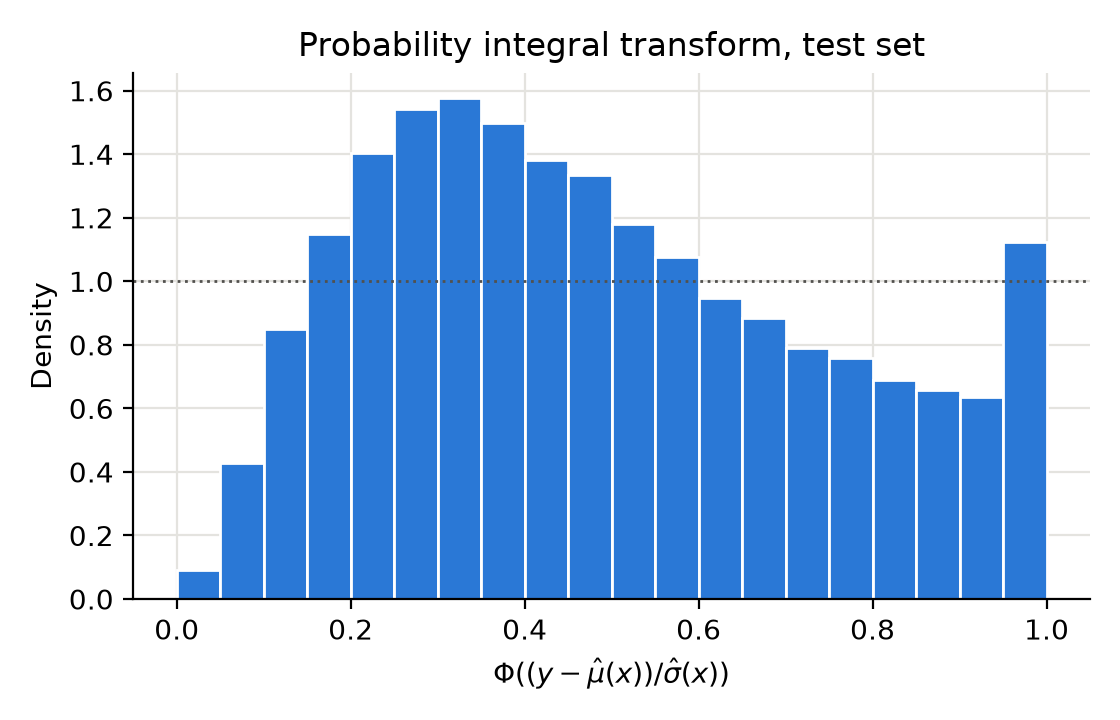
\includegraphics[width=.62\textwidth]{figures/p1_pit.png}\caption{Probability integral transform of test durations under the fitted Gaussian}\end{figure}
\end{enumerate}

\section*{Problem 2}
Code at: \url{https://github.com/aryankaushal06/STAT-37711-A26-PSet-Code/blob/main/PS2/p2.py}

\begin{enumerate}[label=\alph*.]
\item The supplied \texttt{retail.csv} contains $397924$ records, with $3665$ unique stock codes and $4339$ unique customer IDs

One-hot encoding the pair would produce $3665+4339=8004$ indicator columns, with only two active entries per row

This is feasible in a sparse representation, but a dense \texttt{float32} matrix would take $12.74$ GB, and indicators cannot share information across categories, so these features call for target encoding or learned embeddings

The categories are unevenly populated: the median category has $49$ rows for stock codes and $41$ for customers, while $548$ stock codes and $300$ customers have at most $5$ rows

The response is highly right-skewed: its median is $6$, mean $13.02$, standard deviation $180.42$, $99$th percentile $120$, $99.9$th percentile $504$, maximum $80995$, and skewness $403.3$, while $\log(1+y)$ has skewness $0.83$

\begin{figure}[H]\centering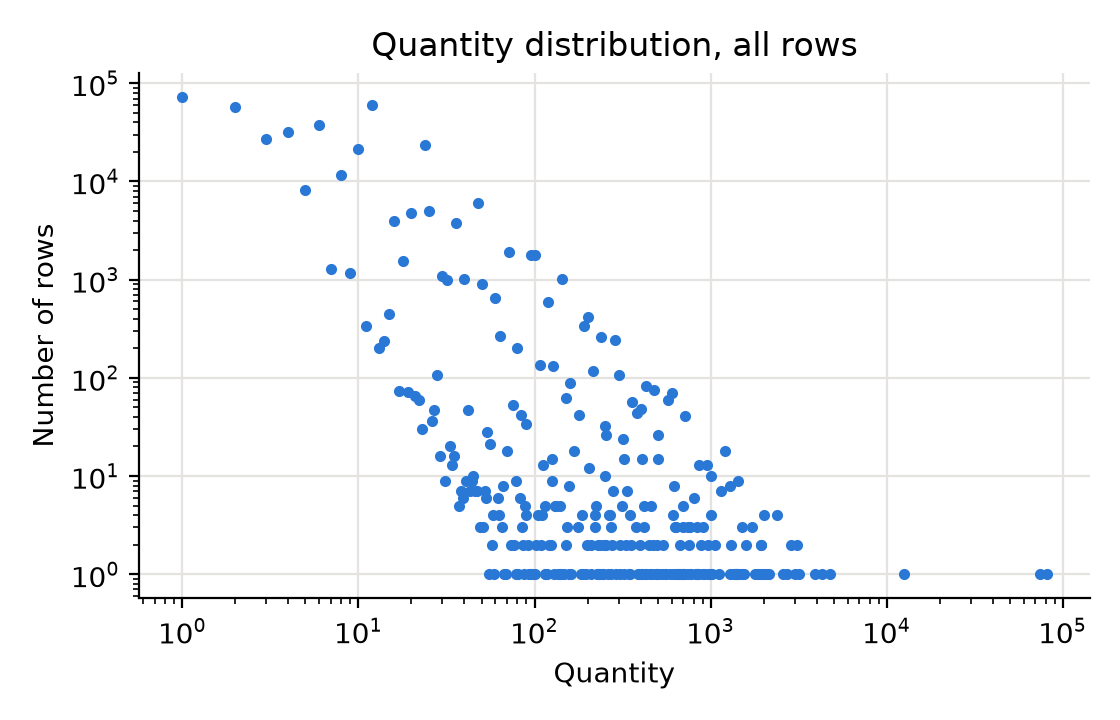
\includegraphics[width=.62\textwidth]{figures/p2_target_distribution.png}\caption{Number of rows at each observed Quantity, on logarithmic axes}\end{figure}

I split the rows randomly with seed $42$, keeping the test partition unused for selection

\begin{table}[H]
\centering
\begin{tabular}{lrrrrr}
\toprule
Split & Rows & Mean & Median & $99$th percentile & Maximum \\
\midrule
Training & 278546 & 13.22 & 6 & 120 & 80995 \\
Validation & 59689 & 12.72 & 6 & 132 & 1930 \\
Test & 59689 & 12.41 & 5 & 120 & 3114 \\
\bottomrule
\end{tabular}
\caption{Quantity by partition}
\end{table}

Only $0.085\%$ of test rows have a stock code unseen in training and $0.027\%$ an unseen customer

The random split lets the same (stock code, customer) pair occur across partitions, since $32.95\%$ of all rows repeat an earlier pair, so these results describe predicting further purchases by known customers and products rather than entirely new ones

Define $t_i=\log(1+y_i)$ to reduce the influence of extreme quantities; models are compared on test MAE of $t$, with RMSE of $t$ and the mean and median absolute error of $y$ alongside it

Predictions of $t$ are clipped to the feasible range $[\log 2,\max\limits_{i\in\mathrm{train}} t_i]$ before scoring

\item I use \texttt{TargetEncoder} from \texttt{category\_encoders} with its default smoothing

For a category $c$ with $n_c$ training rows and category mean $m_c$ of the encoded target, and with overall training mean $\bar m$, the encoding is $e(c)=s_c m_c+(1-s_c)\bar m$, where $s_c=\frac{1}{1+\exp(-(n_c-20)/10)}$

Unseen categories receive $\bar m$, and rare categories shrink toward it

To avoid target leakage, each training row is encoded by an encoder fitted on the other four of five folds, while validation and test rows use an encoder fitted on all training rows

The assignment asks for the mean of the target, so the distinction matters here: the original code encoded the mean of $\log(1+y)$, not the mean of \texttt{Quantity}

The problem permits a target transformation, so I fit both variants, each followed by ridge regression of $t$ on the two encoded features with intercept and $\lambda=10$, and I select between them on validation data

\begin{table}[H]
\centering
\begin{tabular}{lcccc}
\toprule
Encoded quantity & Validation MAE$(t)$ & Test MAE$(t)$ & Test RMSE$(t)$ & Test MAE$(y)$ \\
\midrule
Mean of \texttt{Quantity} & 0.7029 & 0.7019 & 0.8504 & 15.6106 \\
Mean of $\log(1+\texttt{Quantity})$ & \textbf{0.4478} & 0.4440 & 0.6008 & 6.9483 \\
\bottomrule
\end{tabular}
\caption{Target-encoding variants with ridge regression}
\end{table}

Validation selects the $\log(1+y)$ encoding, whose test MAE is $\boxed{0.4440}$ on the log scale and $6.9483$ on the original scale, against $0.8142$ and $10.2068$ for a constant at the training median

The raw mean performs far worse because a category's mean is dominated by its extreme rows; the two largest quantities, $80995$ and $74215$, are both in the training partition

\item I assign each stock code and customer ID an integer index from the training vocabulary, reserving index $0$ for unknown categories

No training row would otherwise use index $0$, leaving unseen test categories with a random untrained vector, so during training I replace each category with index $0$ independently with probability $0.01$

Two separately learned embedding tables map indices into trainable vectors of dimension $\min(32,\max(4,\lceil\sqrt{K}\rceil))$ for a feature with $K$ training categories, which gives dimension $32$ for each feature here; this is far smaller than $K$ while leaving room for several latent properties of a product or customer

Their concatenation passes through a network with hidden widths $64$ and $32$, ReLU activations, and a scalar output predicting $t$

I train with AdamW (learning rate $0.003$, weight decay $0.0001$), batch size $4096$, and smooth-$L_1$ loss with threshold $\beta=0.5$, which limits the influence of remaining outliers

Training runs for at most $100$ epochs, with early stopping on validation loss with patience $5$; the earlier limit of $25$ epochs stopped training while validation loss was still falling

Restoring epoch $40$ of $45$, the model's test log-scale MAE is $\boxed{0.3591}$ and its quantity-scale MAE is $5.8573$

The paired difference from the selected target-encoding model is $-0.0848$ with $95\%$ interval $[-0.0872,-0.0825]$, so the embeddings are clearly better

Since ridge regression minimizes squared error and is a simpler model, I also fit the same MLP and loss on the two encoded features alone; this gives test MAE $0.4258$, so the change of model explains only $0.0182$ of the improvement, and embeddings improve on it by a further $0.0666$ (interval $[-0.0688,-0.0644]$ for the difference)

\item The hybrid model retains the same two embeddings but appends the two out-of-fold target-encoded features, standardized on training rows, before the MLP's first hidden layer; a category replaced by index $0$ also has its encoded feature replaced by the encoding used for unseen categories

The other training settings and the train/validation/test partitions are unchanged

Restoring epoch $23$ of $28$, its test log-scale MAE is $\boxed{0.3599}$ and quantity-scale MAE is $5.9502$

The difference from embeddings alone is $+0.0007$ with paired interval $[-0.0006,0.0020]$, so the hybrid does not improve on them here, and validation MAE points the same way ($0.3600$ against $0.3588$)

\begin{table}[H]
\centering
\begin{tabular}{lccccc}
\toprule
Model & MAE$(t)$ & RMSE$(t)$ & MAE$(y)$ & Median AE$(y)$ & MAE$(t)$ over $3$ seeds \\
\midrule
Target encoding + ridge & 0.4440 & 0.6008 & 6.9483 & 2.0442 & --- \\
Embeddings + MLP & \textbf{0.3591} & \textbf{0.5296} & \textbf{5.8573} & 1.3892 & $0.3590\pm 0.0006$ \\
Hybrid & 0.3599 & 0.5324 & 5.9502 & \textbf{1.3631} & $0.3614\pm 0.0014$ \\
\midrule
Target encoding + MLP & 0.4258 & 0.5911 & 6.6998 & 1.8210 & $0.4251\pm 0.0008$ \\
Constant training median & 0.8142 & 0.9989 & 10.2068 & 4.0000 & --- \\
\bottomrule
\end{tabular}
\caption{Held-out test errors from \texttt{p2.py}; the first four columns use seed $42$, and the last shows mean $\pm$ standard deviation over seeds $42,43,44$ with the same split}
\end{table}

\item \textbf{What the embedding does:} Target encoding supplies a one-dimensional, supervised summary of how a category relates to typical transformed purchase quantity, which directly gives a model a strong signal but collapses all other differences within the category

An embedding instead learns a separate vector for each category by backpropagation, such that two categories can acquire similar representations if doing so improves predictions through the shared downstream network

Because the network sees both vectors jointly, it can represent interactions, such as a customer who buys bulk quantities of only certain kinds of products; a function of two one-dimensional means has little room to express this, which fits the small gain from replacing ridge with an MLP on the encoded features

\textbf{Why the hybrid adds little:} With about $70$ training rows per category on average, the embeddings can learn the information in the encoding themselves

The figure below supports this: the hybrid starts with much lower validation loss, because the encoding is immediately informative, but the two models reach about the same loss within roughly $10$ epochs

The earlier result favoring the hybrid ($0.3554$ against $0.3645$) came from the $25$-epoch limit, which cut off the slower embedding model before it had converged

\begin{figure}[H]\centering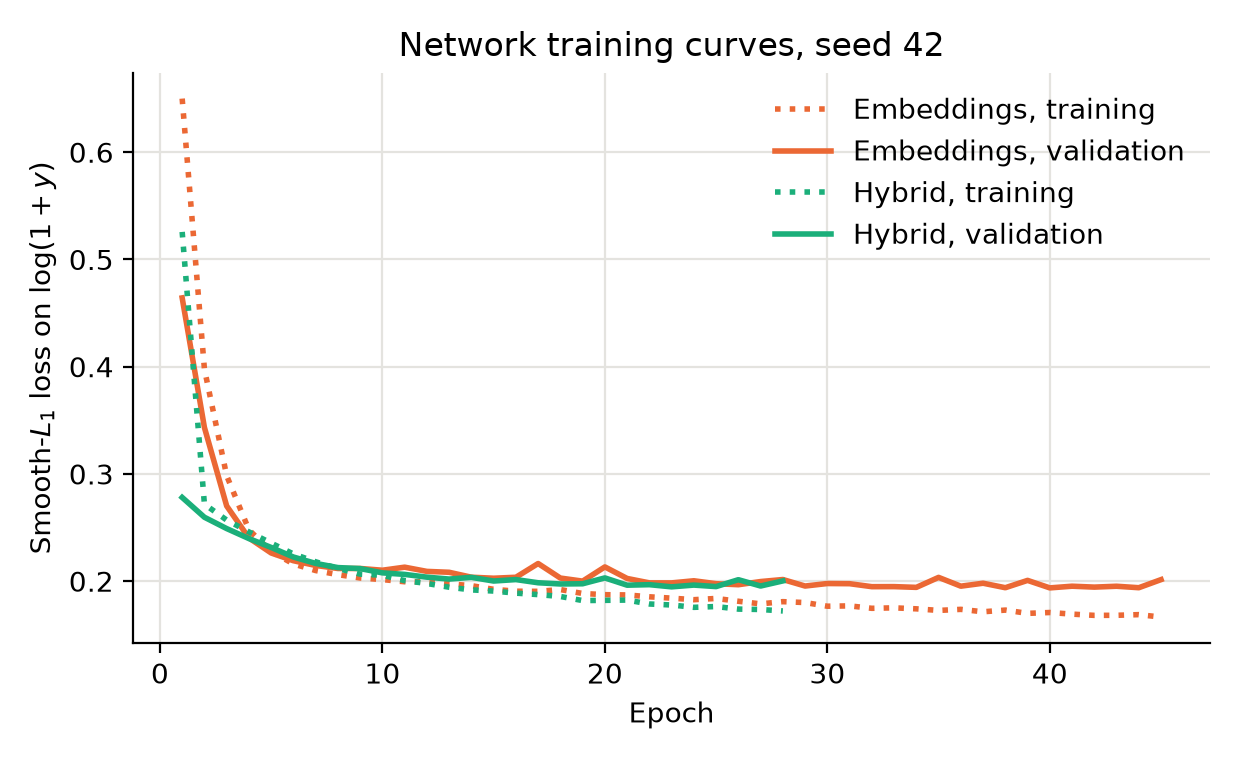
\includegraphics[width=.6\textwidth]{figures/p2_training_curves.png}\caption{Training and validation loss for the embedding and hybrid models, seed $42$}\end{figure}

\textbf{Sparsity and category frequency:} The figure below shows test error by how often a row's category appeared in training

Embedding models beat target encoding in every bin with substantial data, including rare categories: for customers with $1$ to $9$ training rows, MAE is $0.411$ with embeddings and $0.619$ with target encoding

This is consistent with the other feature's embedding compensating for a sparse category, whereas shrinkage moves a rare category's encoding toward an uninformative mean

Unseen customers remain hard for all three models, with MAE near $1.74$ on only $16$ rows, as no method can identify a new customer's purchasing scale from the data available here

\begin{figure}[H]\centering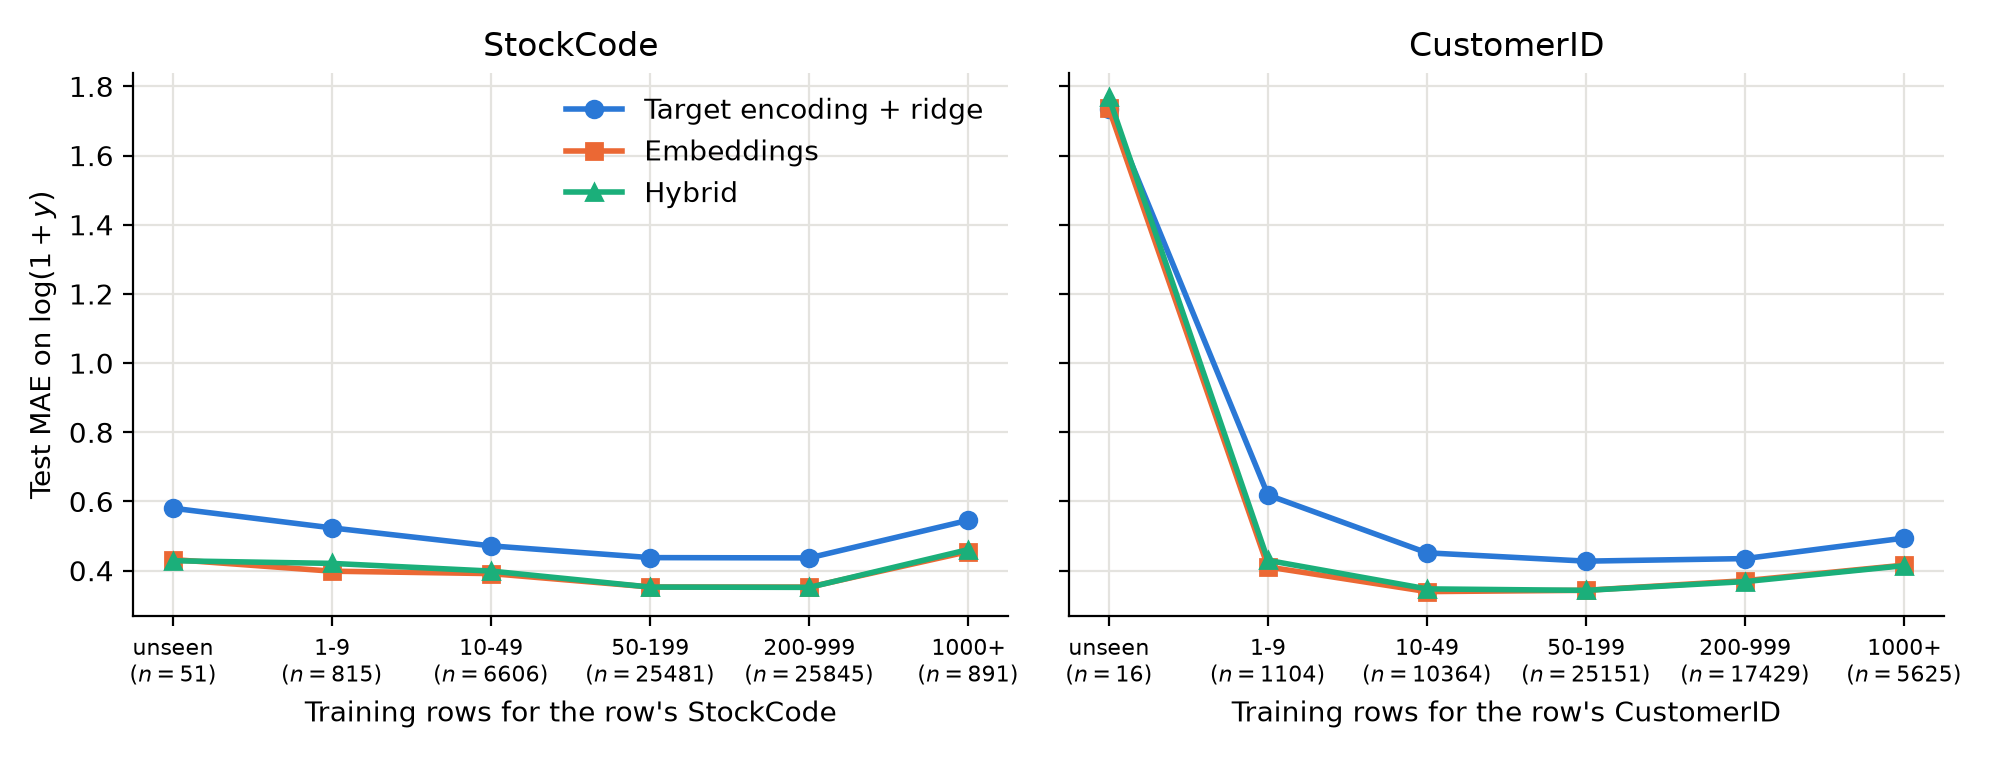
\includegraphics[width=.9\textwidth]{figures/p2_error_by_frequency.png}\caption{Test MAE on $\log(1+y)$ by the number of training rows for each test row's category, with test row counts under each bin}\end{figure}

\textbf{Leakage and generalization:} Encoding a training row with its own target would give the network a feature that is more informative in training than at test time, encouraging overreliance on it; the out-of-fold encoding removes this path, and in the hybrid's training curves the gap between training and validation loss stays small until validation loss flattens

\textbf{Heavy tails:} The log transformation and robust loss target typical purchase sizes, so a prediction $\exp(\hat t)-1$ behaves like a conditional median rather than a conditional mean and will not capture rare bulk orders; the quantity-scale errors should be read accordingly

\textbf{Limitations:} The confidence intervals treat fitted models as fixed and reflect only test sampling variation, the seed comparison uses one split and one set of hyperparameters, and the hybrid could gain with different regularization or in a setting with fewer rows per category, none of which I tested
\end{enumerate}

\section*{Problem 3}
Code at: \url{https://github.com/aryankaushal06/STAT-37711-A26-PSet-Code/blob/main/PS2/p3.py}

\begin{enumerate}[label=\alph*.]
\item The supplied split consists of $600$ training, $200$ validation, and $200$ unlabeled test points, with two features $x_1,x_2\in[-3,3]$

The training visualizations below show the response $y$ as color at each input location and as height in three dimensions, exposing a smooth but nonlinear response

The response is lowest near $(x_1,x_2)=(-1.5,0)$, highest near the edges $x_2=\pm 3$ around $x_1=1.5$, and appears roughly symmetric in $x_2$

\begin{figure}[H]\centering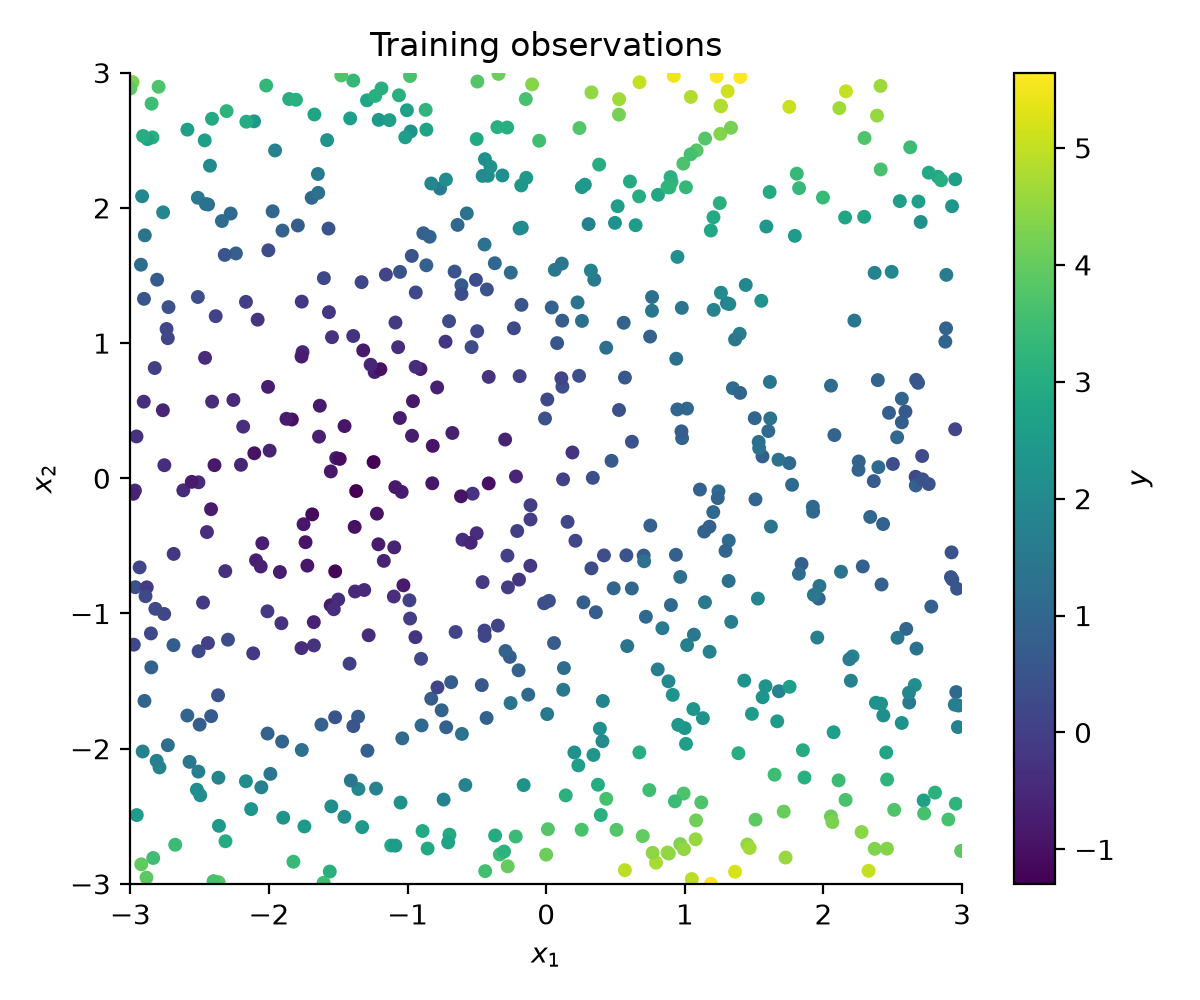
\includegraphics[width=.48\textwidth]{figures/p3_train.png}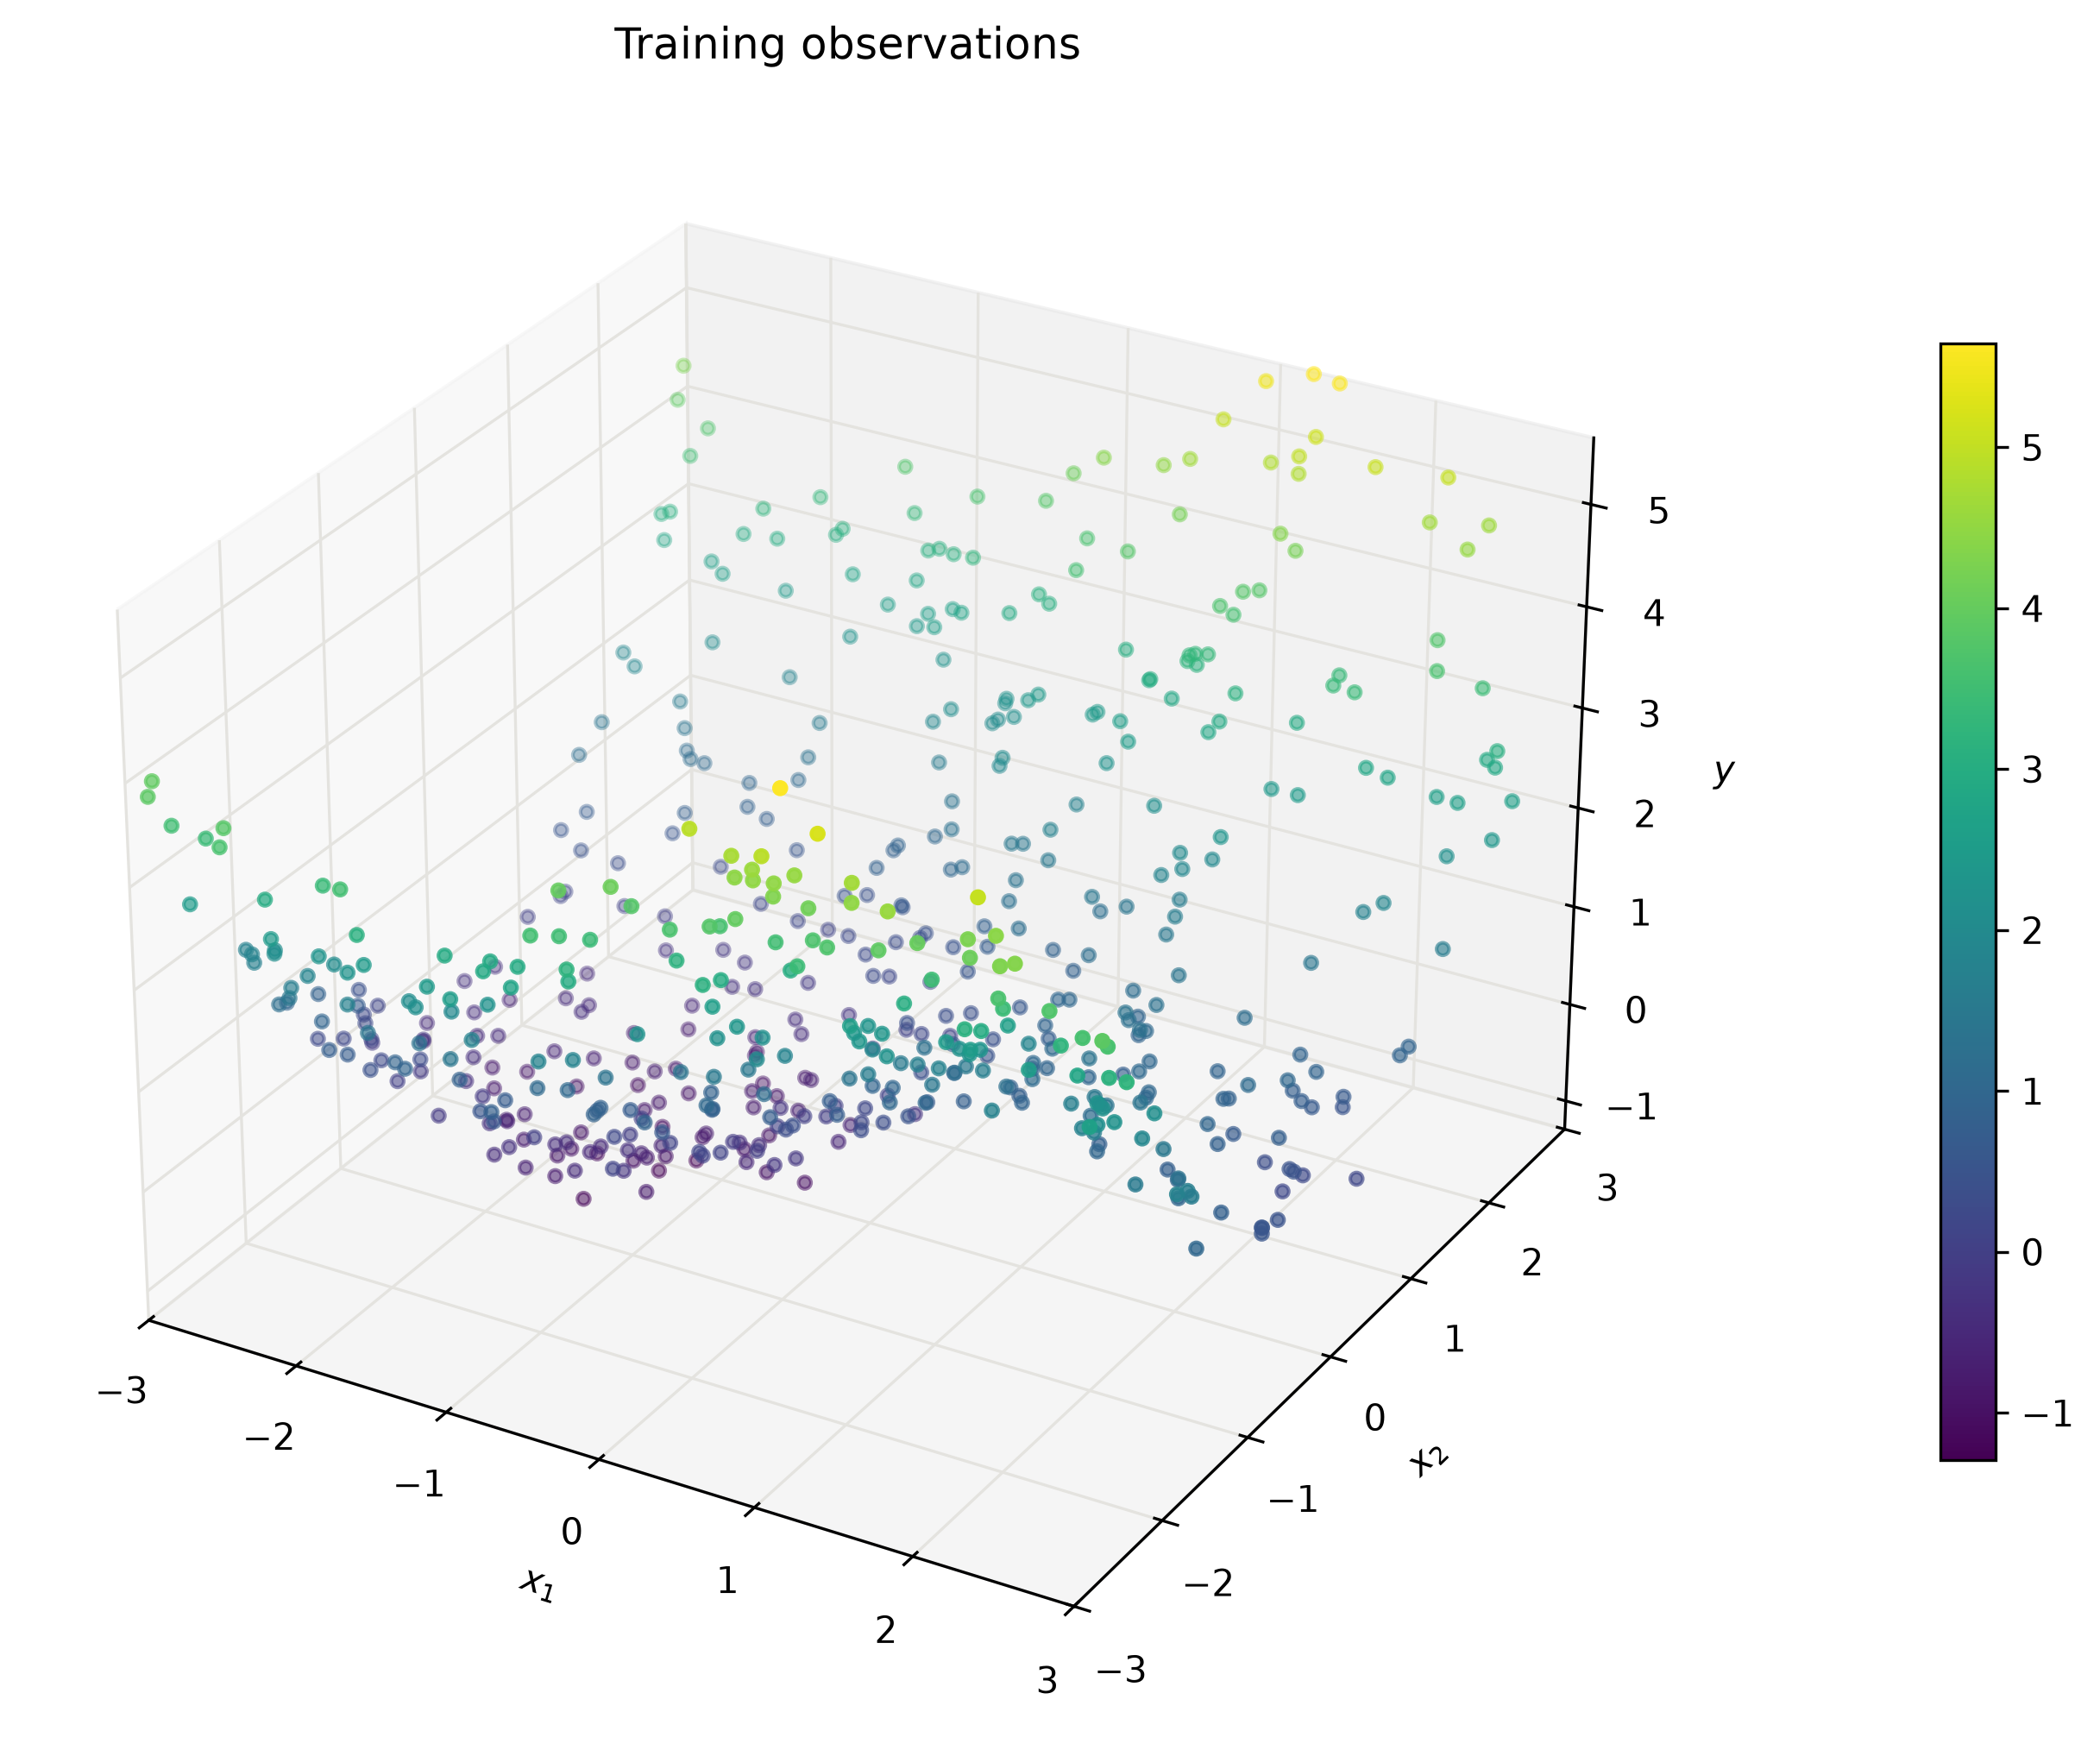
\includegraphics[width=.48\textwidth]{figures/p3_train_3d.png}\caption{Training response as a function of the two covariates, by color (left) and in three dimensions (right)}\end{figure}

\item For each even number $D=2h$, I sample $w_j\overset{\mathrm{iid}}\sim\mathcal N_2(0,I_2/\sigma^2)$ and $b_j\overset{\mathrm{iid}}\sim\operatorname{Unif}[0,2\pi]$ for $j=1,\ldots,h$ with seed $42$

The map is exactly the assignment's $z(x)=(\sin(w_1^Tx+b_1),\cos(w_1^Tx+b_1),\ldots,\sin(w_h^Tx+b_h),\cos(w_h^Tx+b_h))^T\in\mathbb R^D$; I removed an additional $\frac{1}{\sqrt h}$ factor from the original code, which made the effective penalty depend on $h$

Each larger $D$ extends the same sequence of draws, so the sweep varies $D$ without also drawing an unrelated set of features

For design matrix $Z$ with rows $z(x_i)^T$ and mean training response $\bar y$, I minimize $\|y-\bar y\mathbf 1-Z\beta\|_2^2+\lambda\|\beta\|_2^2$

The unique solution is $\hat\beta=(Z^TZ+\lambda I_D)^{-1}Z^T(y-\bar y\mathbf 1)$ since $\lambda>0$ makes the matrix positive definite; the implementation solves this linear system without computing a matrix inverse explicitly

I hold $\lambda=1$ and $\sigma=3.079$ fixed, where $\sigma$ is the median pairwise distance among training inputs (the median heuristic), and $\lambda=1$ gives light regularization that keeps the system well conditioned when $D>n$

I sweep $D\in\{10,20,50,100,200,400,800,1600\}$ and select the minimum validation MSE

\begin{table}[H]\centering\begin{tabular}{rccc}\toprule $D$ & Training MSE & Validation MSE & Validation MSE over $5$ seeds \\\midrule
10 & 0.24682 & 0.23286 & $0.26569\pm 0.09309$ \\
20 & 0.16858 & 0.16829 & $0.17176\pm 0.04380$ \\
50 & 0.04138 & 0.04277 & $0.05292\pm 0.00913$ \\
100 & 0.03847 & 0.03931 & $0.04333\pm 0.00268$ \\
200 & 0.03722 & 0.03816 & $0.03734\pm 0.00062$ \\
400 & 0.03539 & 0.03639 & $0.03626\pm 0.00023$ \\
800 & 0.03390 & \textbf{0.03585} & $0.03587\pm 0.00013$ \\
1600 & 0.03328 & 0.03602 & $0.03597\pm 0.00006$ \\
\bottomrule\end{tabular}\caption{RKS hyperparameter sweep; the first two error columns use seed $42$, and the last shows mean $\pm$ standard deviation over seeds $42$ to $46$}\end{table}

The selected model has $\boxed{D=800}$ and validation MSE $\boxed{0.03585}$

Training MSE falls throughout, while validation MSE flattens beyond $D=400$ and rises slightly at $D=1600$, so the choice among the largest values is not sharply determined

\begin{figure}[H]\centering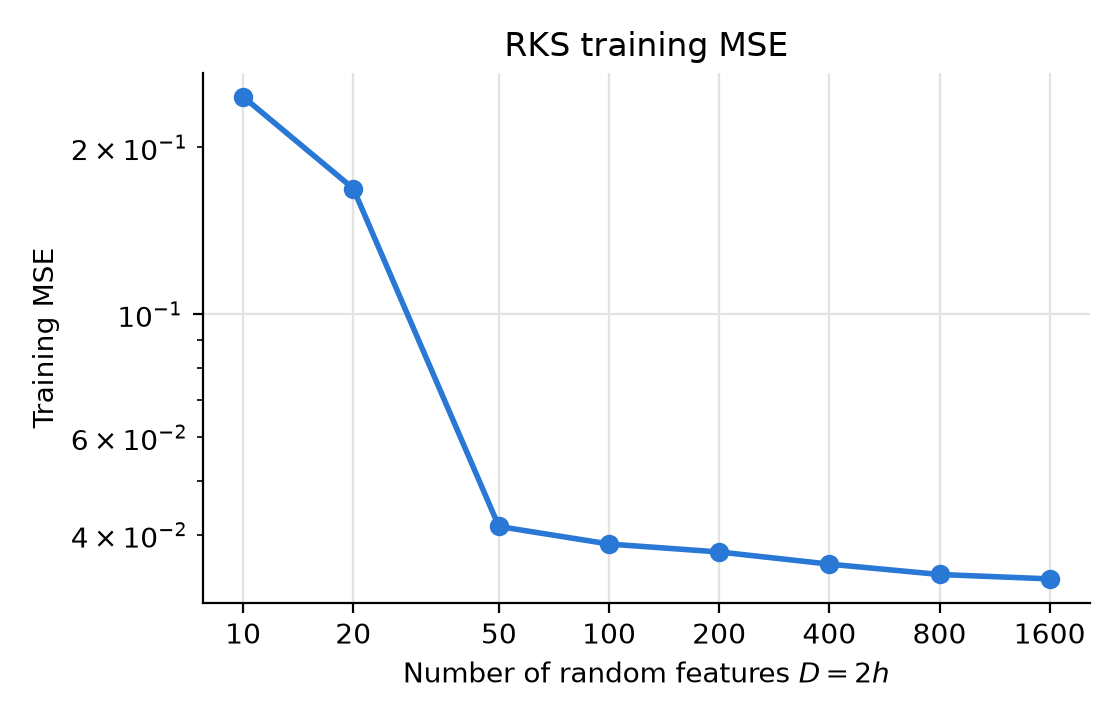
\includegraphics[width=.48\textwidth]{figures/p3_rks_train.png}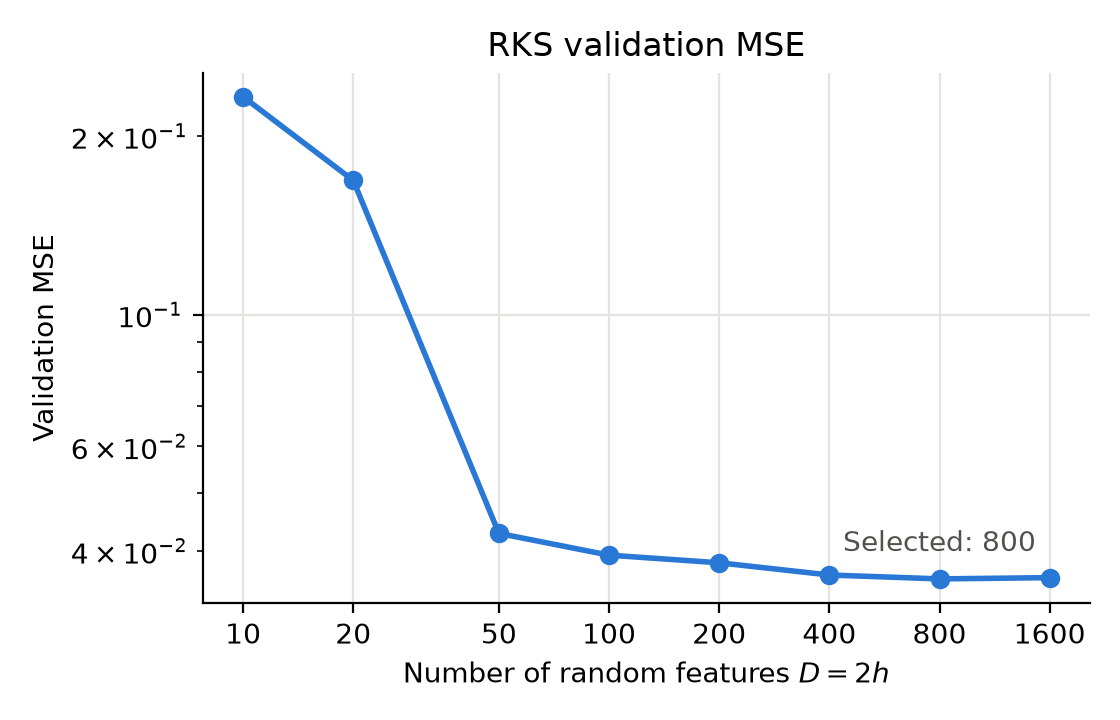
\includegraphics[width=.48\textwidth]{figures/p3_rks_val.png}\caption{RKS training and validation MSE over feature count $D$, on logarithmic axes}\end{figure}

At $D=800$, mean validation MSE over the same five seeds is $0.0359$ to $0.0384$ at $\sigma=3.079$ for $\lambda\in\{0.01,0.1,1,10\}$, $0.0368$ to $0.0376$ at $\sigma=2$, $0.0397$ to $0.0435$ at $\sigma=1$, and $0.0440$ to $0.0533$ at $\sigma=0.5$

I inspected these validation values before fixing $\sigma$ and $\lambda$, so the reported validation MSE may be mildly optimistic

\item The one-hidden-layer MLP has the form $f_\theta(x)=v^T\tanh(Wx+a)+c$, with $W\in\mathbb R^{h\times2}$, $a,v\in\mathbb R^h$, and scalar $c$

I minimize training MSE with full-batch Adam, initial learning rate $0.01$ with cosine decay to $0$, for $5000$ epochs, with seed $42$

I vary hidden width $h\in\{8,16,32,64,128\}$ while holding the remaining choices constant, and I no longer select an epoch per width using validation data, so that width is the only quantity chosen on the sweep

The original $300$ epochs at constant learning rate left the models underfit, with training MSE of $0.04322$ and validation MSE of $0.04549$ at $h=128$ and $0.12919$ and $0.13205$ at $h=8$, so that sweep mainly measured optimization speed

\begin{table}[H]\centering\begin{tabular}{rccc}\toprule $h$ & Training MSE & Validation MSE & Validation MSE over $5$ seeds \\\midrule
8 & 0.03354 & 0.03858 & $0.03985\pm 0.00252$ \\
16 & 0.03259 & \textbf{0.03555} & $0.03697\pm 0.00089$ \\
32 & 0.03132 & 0.03801 & $0.03755\pm 0.00065$ \\
64 & 0.03027 & 0.03807 & $0.03791\pm 0.00033$ \\
128 & 0.02995 & 0.03799 & $0.03757\pm 0.00060$ \\
\bottomrule\end{tabular}\caption{One-hidden-layer MLP sweep; the first two error columns use seed $42$, and the last shows mean $\pm$ standard deviation over seeds $42$ to $46$}\end{table}

The selected MLP has $\boxed{h=16}$ and validation MSE $\boxed{0.03555}$

Training MSE falls with width while validation MSE does not; the seed-$42$ value at $h=16$ is below that width's mean over seeds, so part of this minimum is favorable initialization, although $h=16$ also has the lowest mean

\begin{figure}[H]\centering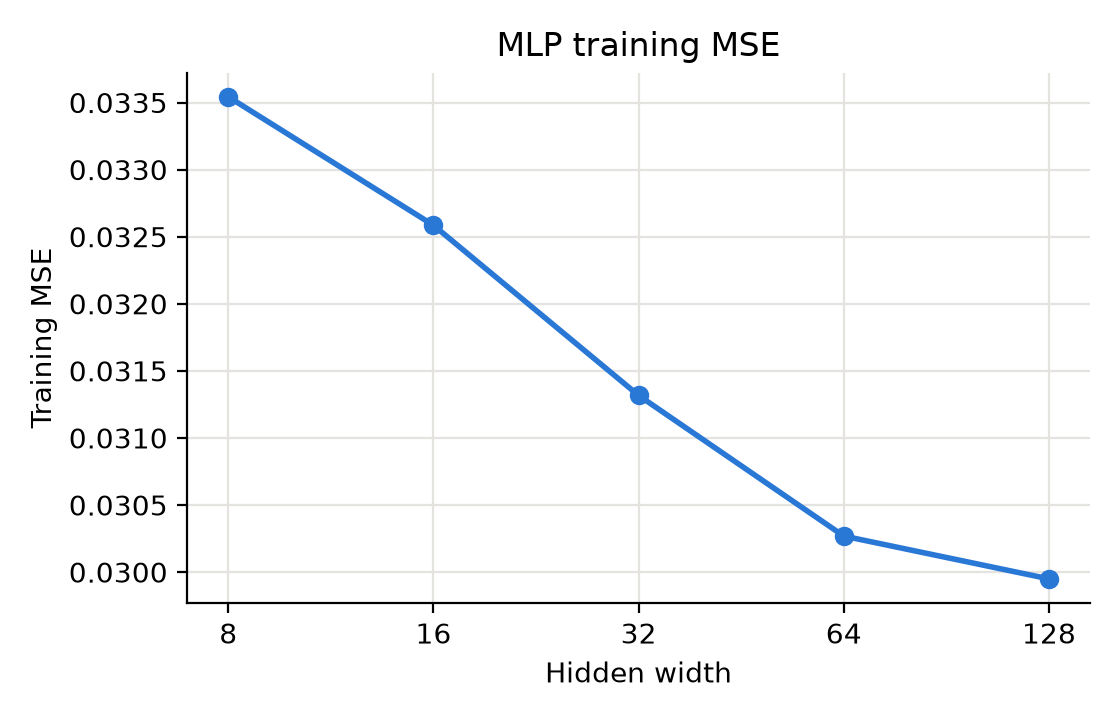
\includegraphics[width=.48\textwidth]{figures/p3_mlp_train.png}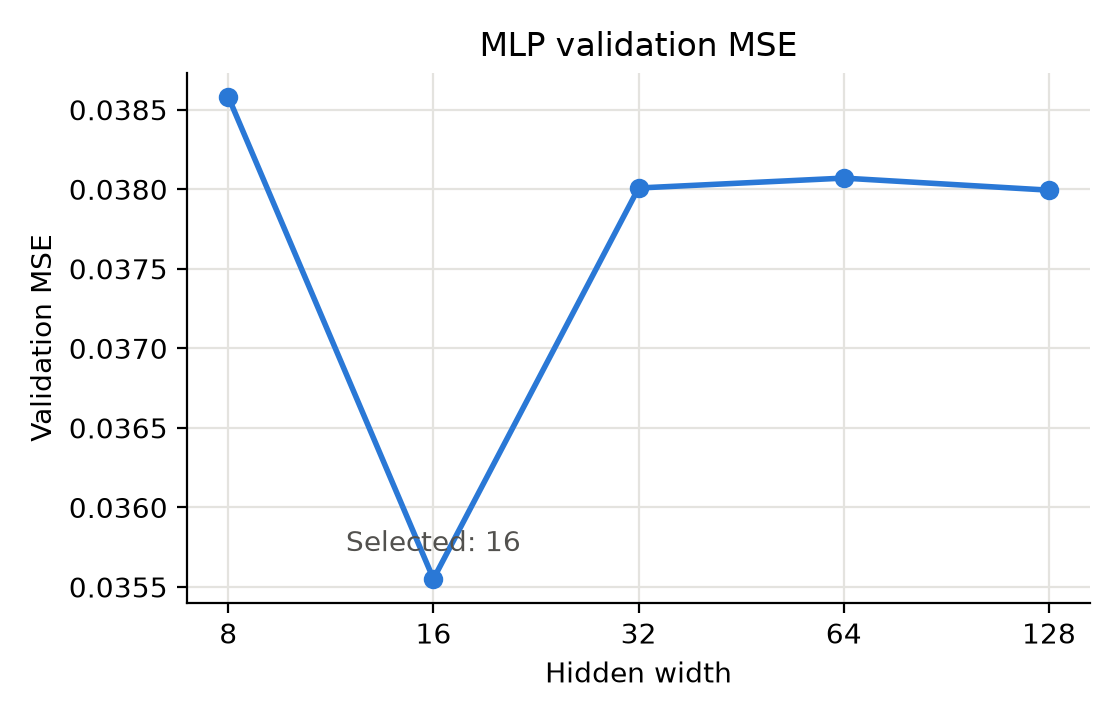
\includegraphics[width=.48\textwidth]{figures/p3_mlp_val.png}\caption{MLP training and validation MSE over hidden width, on a logarithmic width axis}\end{figure}

\item Refitting at the selected values reproduces the sweep: RKS achieves validation MSE $0.03585$ and the MLP $0.03555$

The MLP is lower by $0.00030$, but the paired $95\%$ interval for the difference (RKS minus MLP) over the $200$ validation points is $[-0.00160,0.00220]$, so the data do not separate the two models

Over seeds the order reverses: $0.03587\pm 0.00013$ for RKS at $D=800$ and $0.03697\pm 0.00089$ for the MLP at $h=16$

I therefore conclude that the two perform about equally, with the RKS result more stable across seeds

This changes the conclusion of the original implementation, whose apparent RKS advantage ($0.03690$ against $0.04510$) reflected the underfit MLP

The two models differ in how they obtain features: RKS fixes random sinusoids and solves a convex ridge problem with a unique solution given the draw, so it needs many features ($800$ coefficients) to cover the relevant directions and frequencies, and its variation across seeds shrinks as $D$ grows

The MLP learns its features through a nonconvex problem, which lets $h=16$ with only $4h+1=65$ parameters adapt its units to this response, at the cost of sensitivity to initialization and the optimization budget, as the $300$-epoch result shows

Both surfaces below use the same grid over $[-3,3]^2$, color scale, vertical range, and viewing angle

\begin{figure}[H]\centering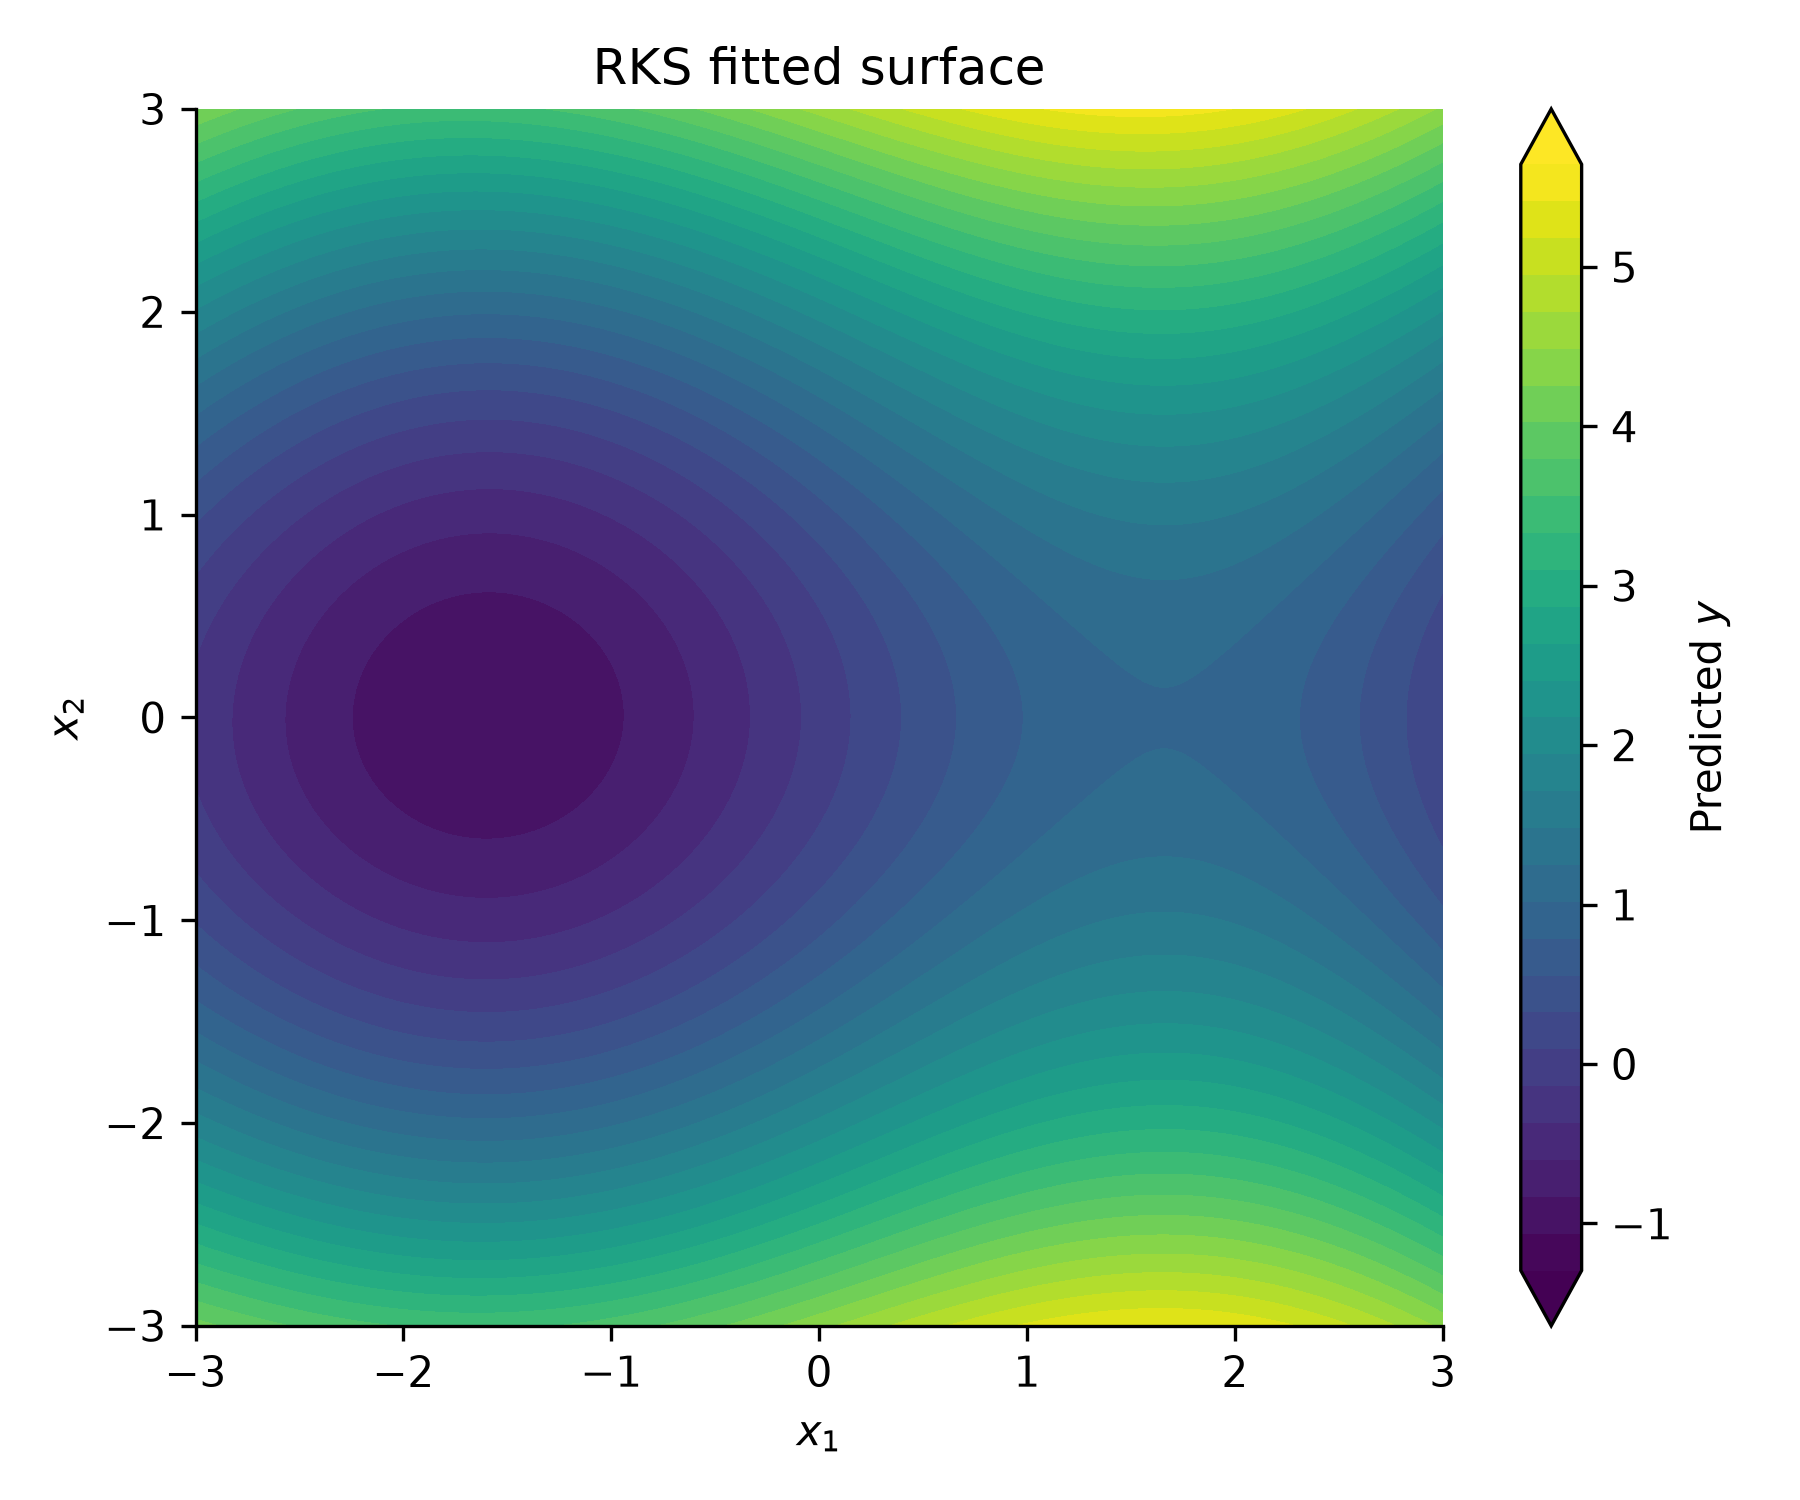
\includegraphics[width=.48\textwidth]{figures/p3_rks_surface.png}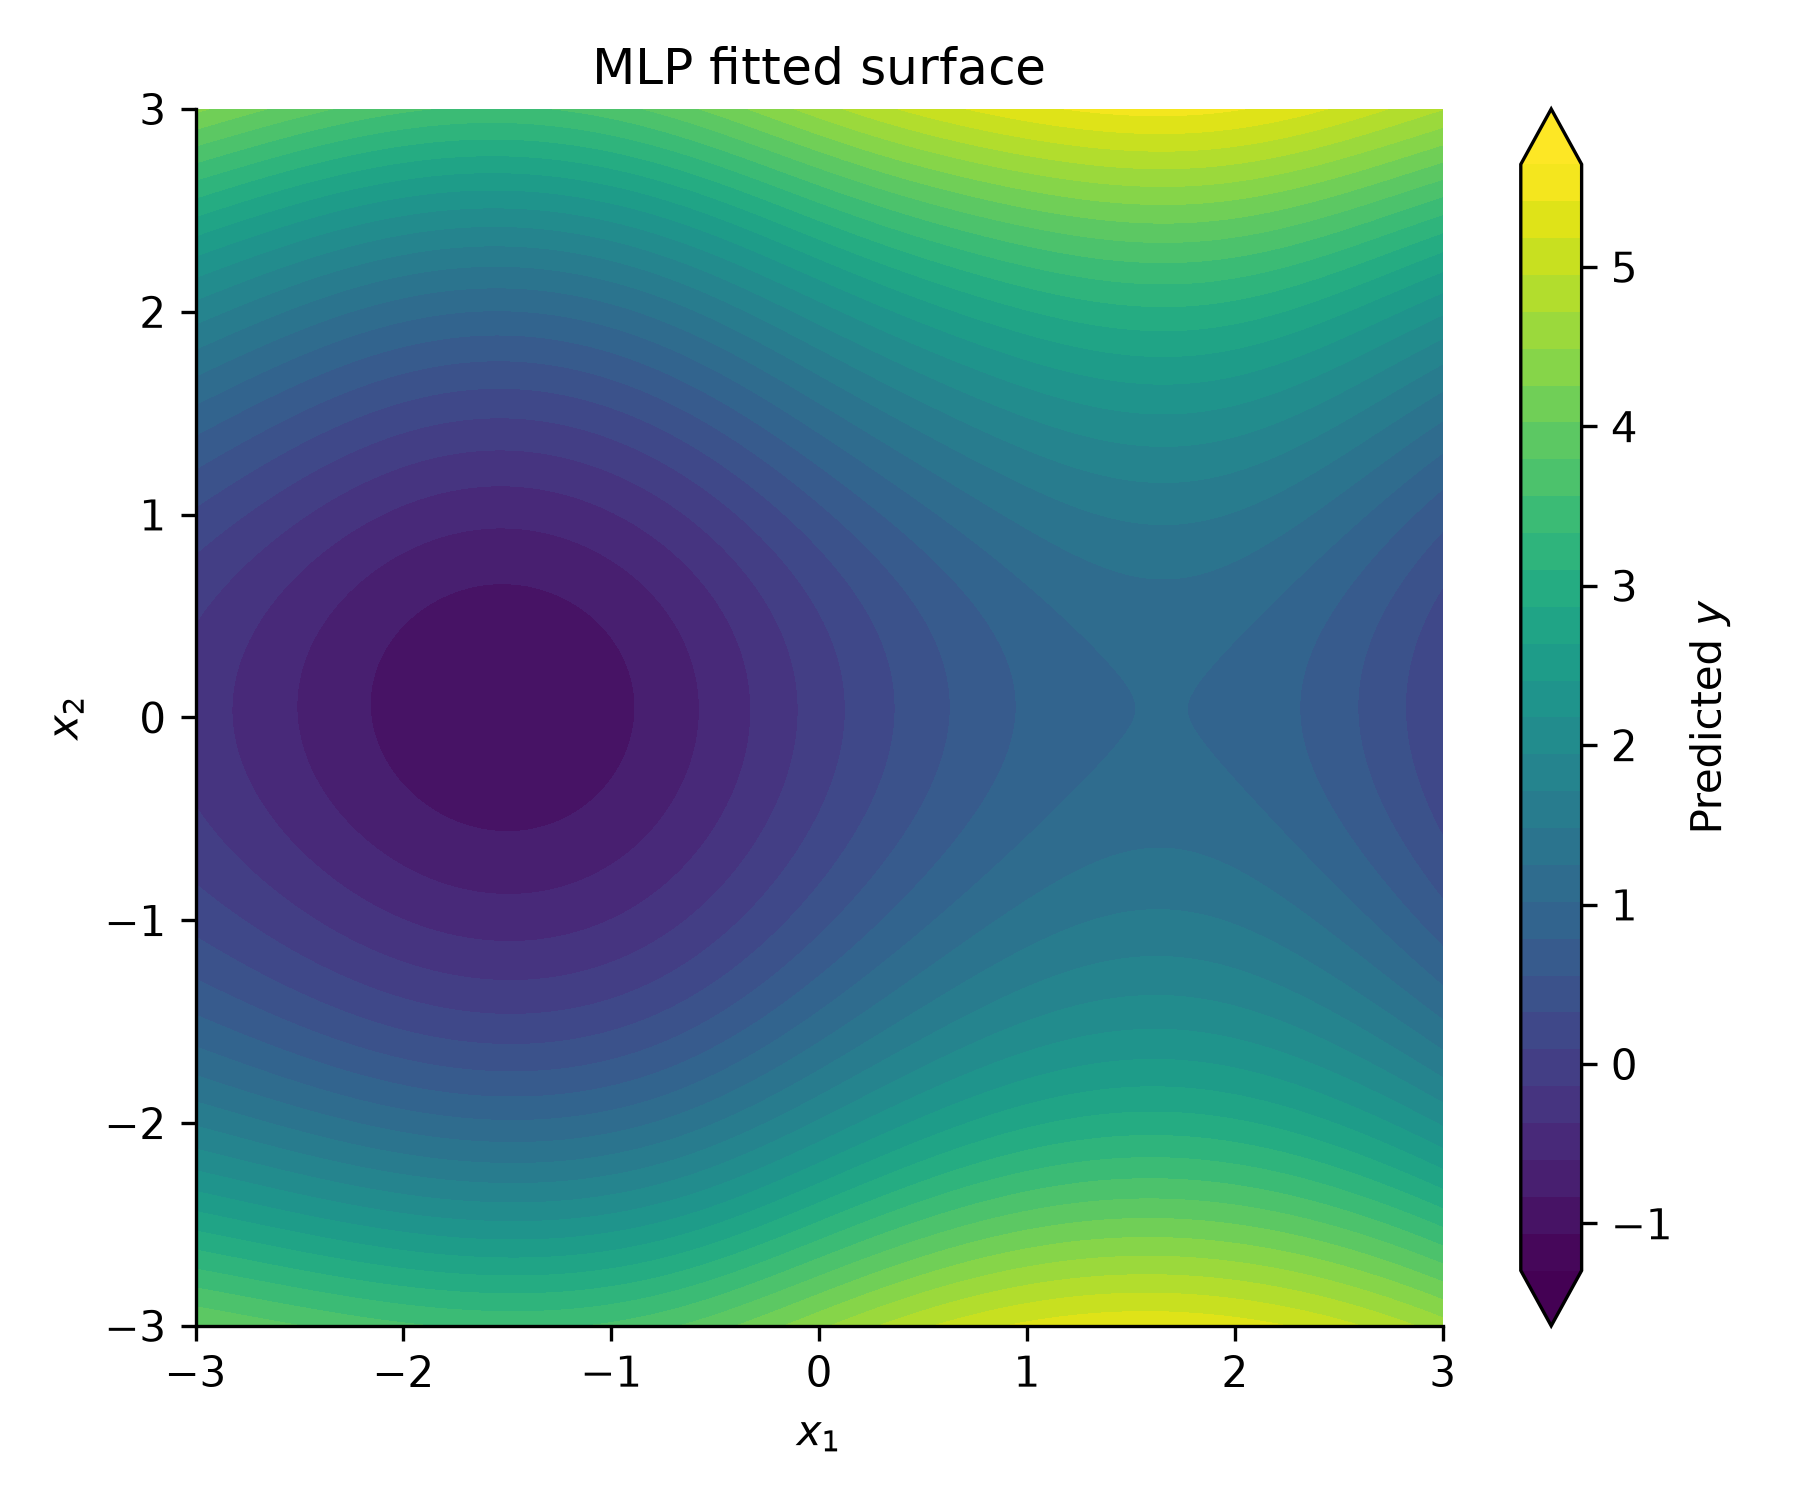
\includegraphics[width=.48\textwidth]{figures/p3_mlp_surface.png}\caption{Fitted surfaces from selected RKS (left) and MLP (right), on a common color scale}\end{figure}

\begin{figure}[H]\centering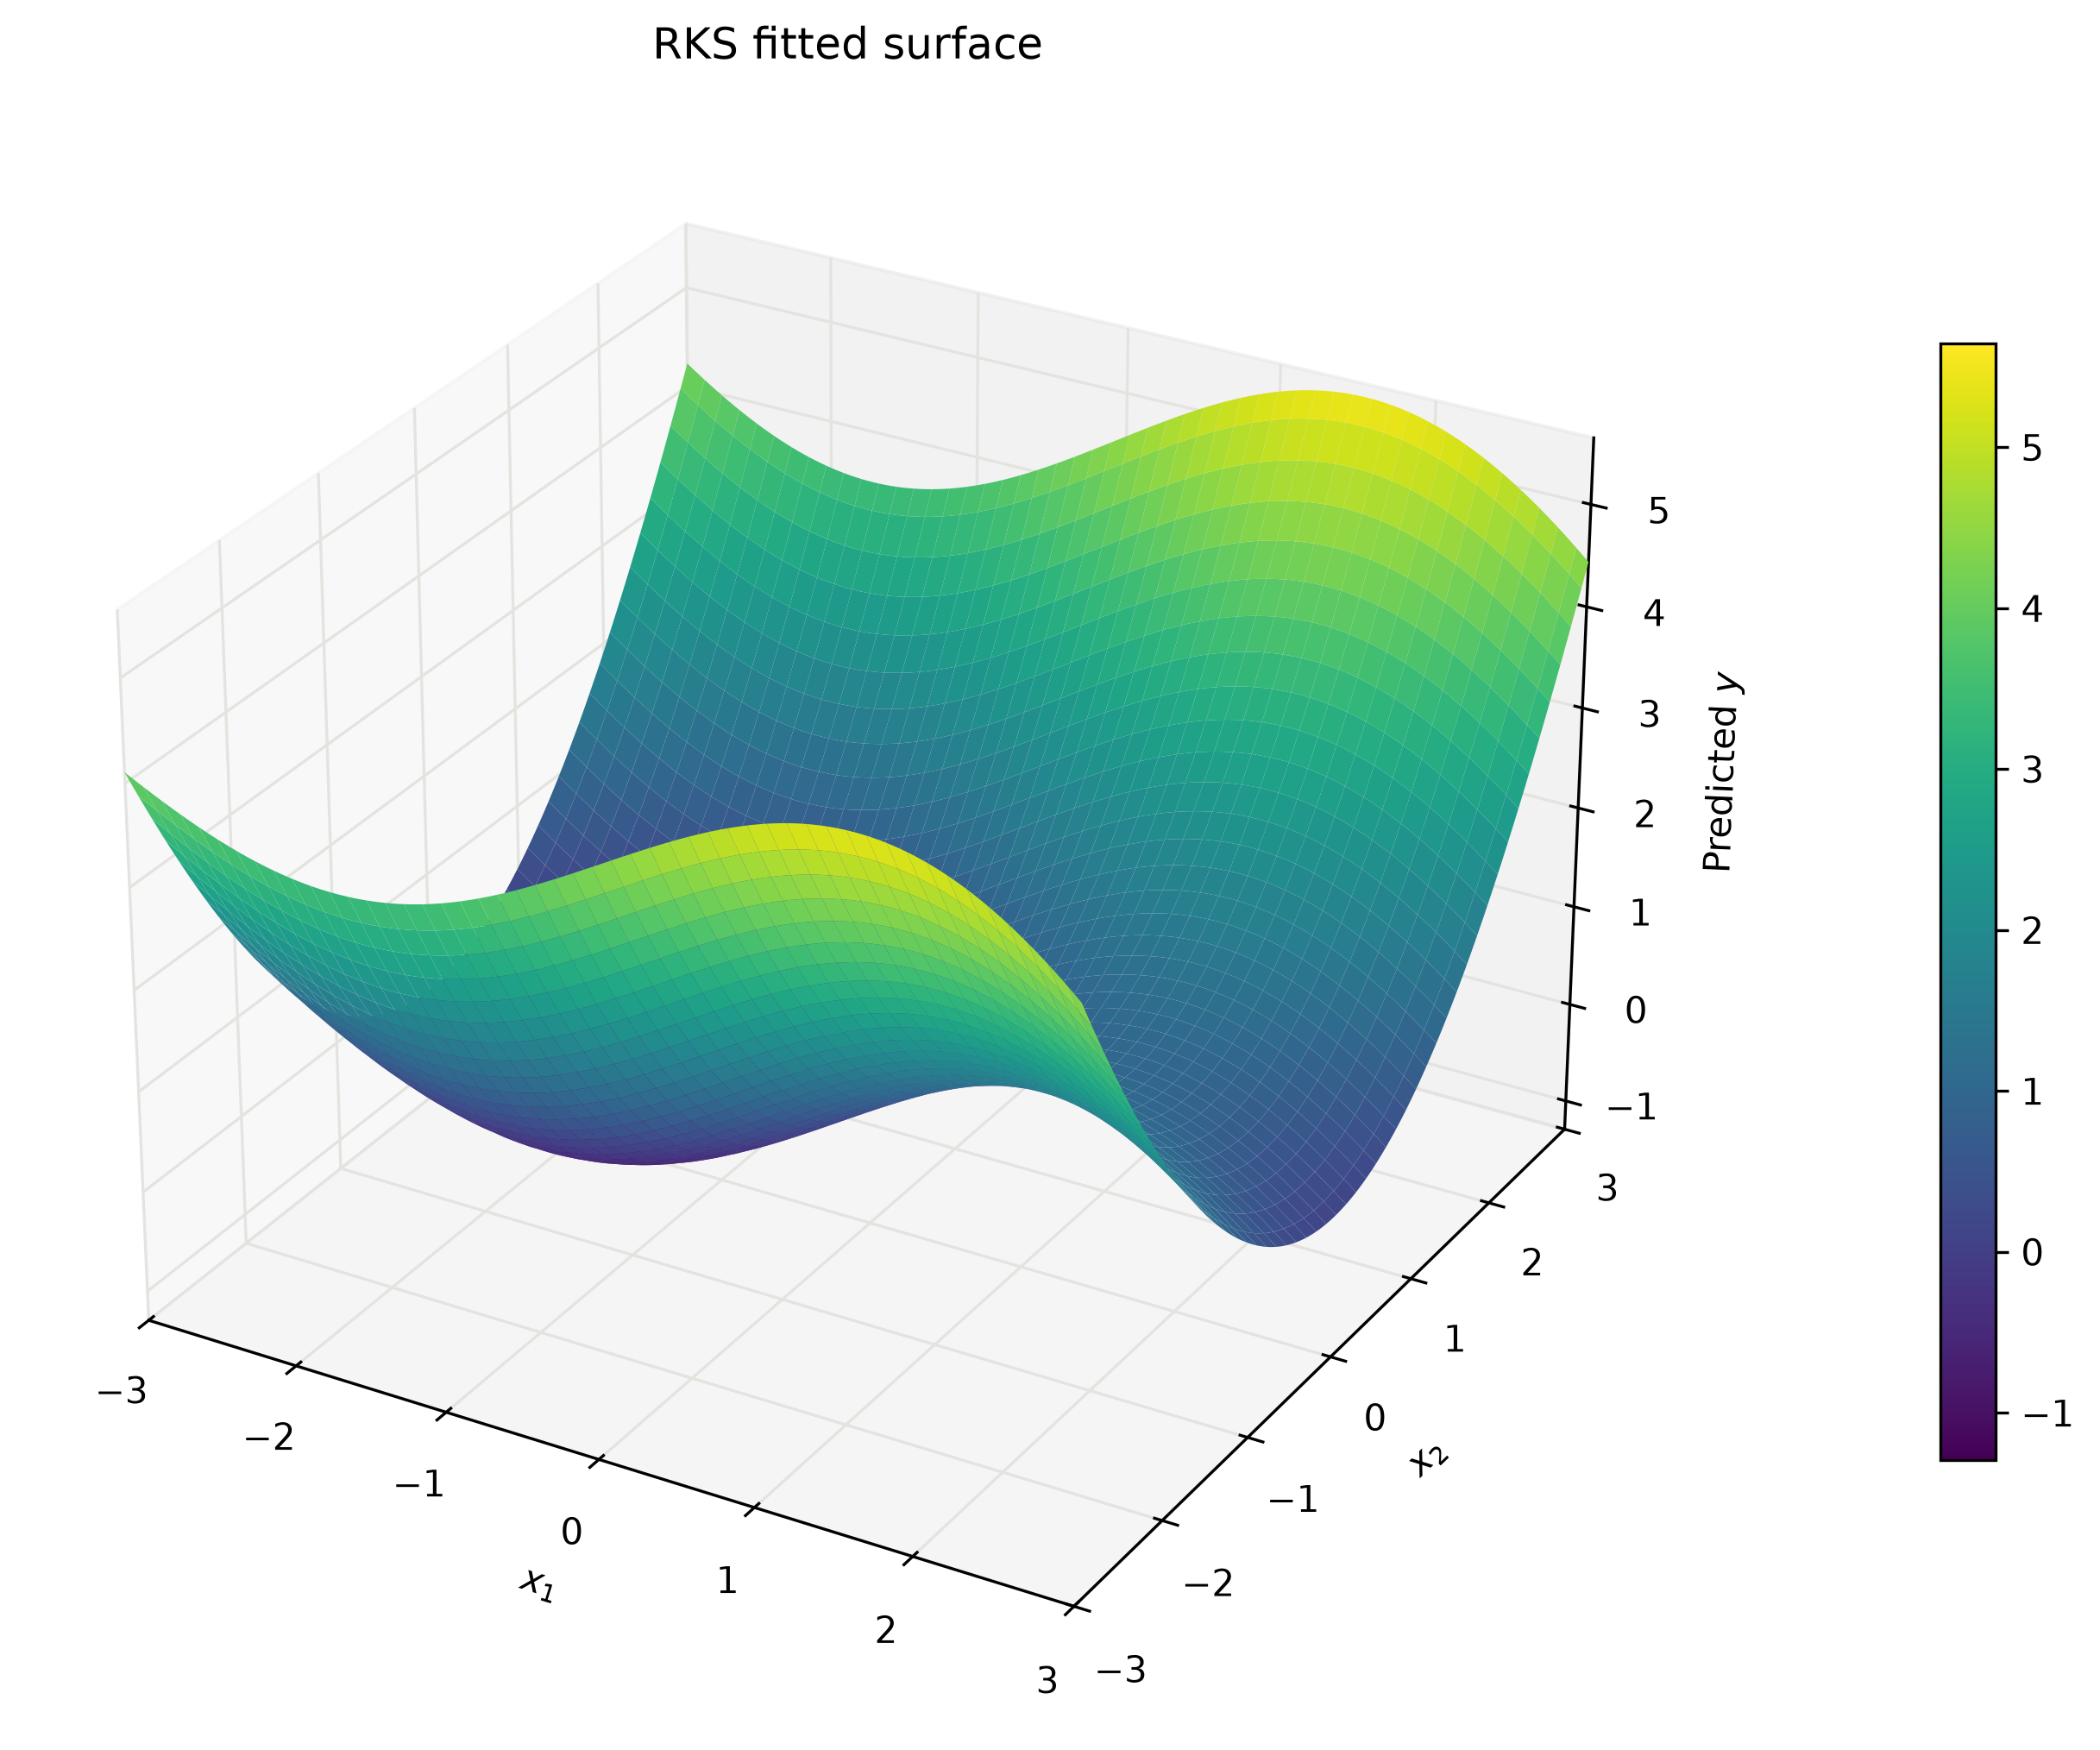
\includegraphics[width=.48\textwidth]{figures/p3_rks_surface_3d.png}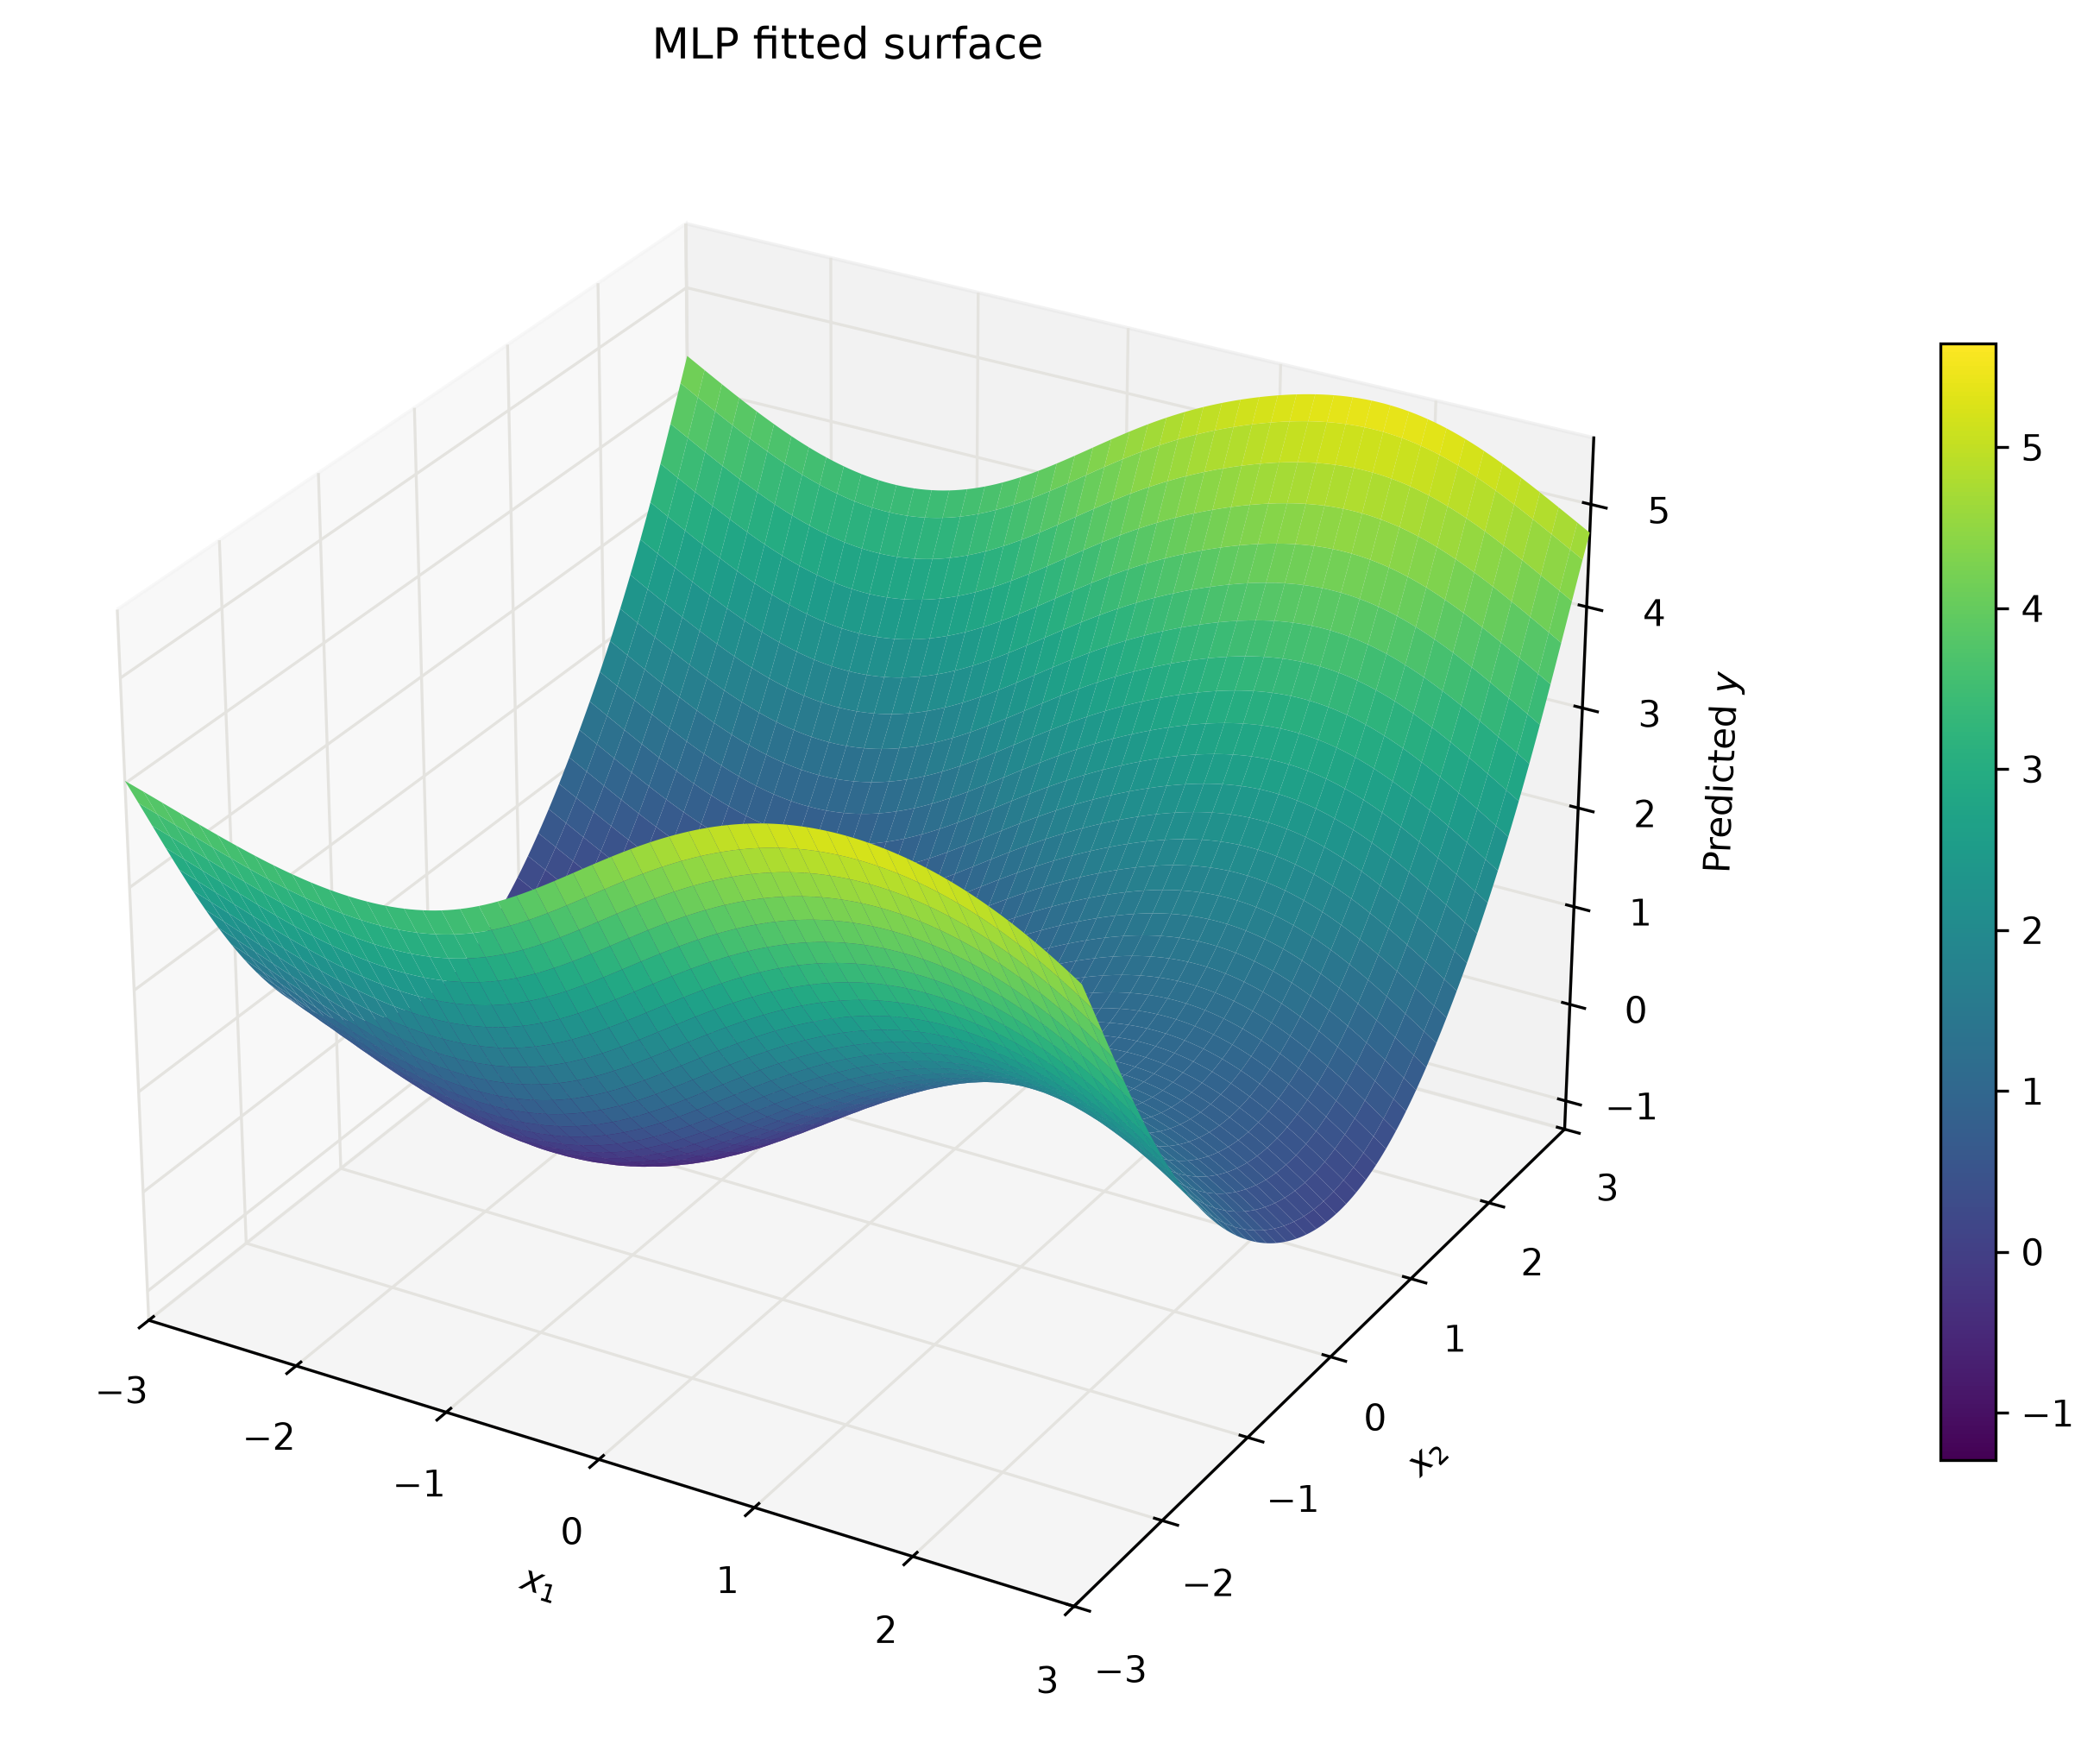
\includegraphics[width=.48\textwidth]{figures/p3_mlp_surface_3d.png}\caption{Three-dimensional fitted surfaces from selected RKS (left) and MLP (right), with identical axes, color scale, and viewing angle}\end{figure}

Both models recover the structure seen in part (a): a basin with its minimum near $(-1.6,0)$ (at $(-1.59,0.02)$ for RKS and $(-1.51,0.06)$ for the MLP, with values $-1.03$), a saddle near $(1.6,0)$ with a smaller depression toward $x_1=3$, and maxima on the edge $x_2=3$ near $x_1=1.6$ (values $5.52$ and $5.50$)

The two surfaces are nearly identical, with mean absolute difference $0.028$ on the grid, and they differ most at the boundary, reaching their maximum difference of $0.286$ at the corner $(3,3)$, where few training points constrain either fit

The agreement is consistent with the near-equal validation errors

Finally, I used each selected configuration, fitted on the supplied labeled training set, to predict the $200$ unlabeled rows of \texttt{test.csv} in their original order

The required files are \texttt{rks\_test\_predictions.csv} and \texttt{mlp\_test\_predictions.csv}, each headerless with one prediction per row; test MSE cannot be computed because the test targets are intentionally withheld
\end{enumerate}
\end{document}
